\documentclass{article}

\makeatletter
\renewcommand{\fnum@figure}{Εικόνα \thefigure}
\makeatother

\usepackage[greek, english]{babel}
\usepackage{alphabeta}
\usepackage{atbegshi, picture}

% Set page size and margins
% Replace `letterpaper' with`a4paper' for UK/EU standard size
\usepackage[letterpaper,top=2cm,bottom=2cm,left=3cm,right=3cm,marginparwidth=1.75cm]{geometry}

% Useful packages
\usepackage{amsmath}
\usepackage{graphicx}
\usepackage[colorlinks=true, allcolors=blue]{hyperref}
\usepackage[utf8]{inputenc}
\usepackage{indentfirst}

\addto\captionsenglish{
  \renewcommand{\contentsname}
    {Περιεχόμενα}
}

% \title{Feasibility Study}
% \date{}

\begin{document}
% \maketitle

\begin{titlepage}
   \begin{center}
       \vspace*{1cm}

       \textbf{\huge Project Description}

       \vspace{0.5cm}
        Τεχνολογία Λογισμικού
            
       \vspace{1cm}

       \textbf{Κατερίνα Μητροπούλου\\Μάριος Στεφανίδης}
       
       \begin{figure}[!htb]
        \centering
        
\includegraphics[width=0.5\textwidth]{logo.png}
        \end{figure}
        
        \vspace{0.5cm}
        
        \begin{figure}[!htb]
        \centering
        \includegraphics[width=0.5\textwidth]{UoP.jpg}
        \end{figure}


       \vfill
            
       Τεχνικό Κείμενο για την Τεχνολογία Λογισμικού\\
            
       \vspace{0.5cm}
            
       CEID, ECE\\
       University of Patras\\
            
   \end{center}
\end{titlepage}



\noindent Η ομάδα μας

\begin{enumerate}
  \item Βεργίνης Δημήτριος, ΑΜ: 1066634 , ECE
  \item Βλαχογιάννης Δημήτριος, ΑΜ: 1067371, CEID
  \item Κούρου Αγγελική, ΑΜ: 1067499 , CEID
  \item Μητροπούλου Αικατερίνα - Quality Manager, ΑΜ: 1067409, CEID
  \item Στεφανίδης Μάριος - Project Manager, ΑΜ:1067458, CEID
\end{enumerate}

{
  \hypersetup{linkcolor=black}
  \tableofcontents
}

\section{Εισαγωγή}
    Στο συγκεκριμένο τεχνικό κείμενο θα δοθεί μια αρχική περιγραφή του έργου που θα υλοποιήσει η ομάδας μας σε φυσική γλώσσα χωρίς τη χρήση τεχνικών όρων και την αναφορά σε τεχνικές και σχεδιαστικές λεπτομέρειες. Επιπλέον, θα παρουσιαστούν κάποια ενδεικτικά mock-up screens ή διαφορετικά κάποιες από τις βασικές οθόνες που θα περιλαμβάνει η εφαρμογή μας, που θα επιδεικνύουν τις λειτουργίες της. \par
    Η ομάδα μας θα προσπαθήσει να δημιουργήσει ένα λογισμικό βασιζομένη στον ανθρωποκεντρικό σχεδιασμό λαμβάνοντας υπόψιν βασικές μεθόδους αξιολόγησης (expert evaluation), όπως είναι οι 10 κανόνες του Nielsen και Molich (Heuristic Evaluation), 
    το Cognitive Walkthrough κλπ, ώστε η εφαρμογή που θα προκύψει, να είναι εύχρηστη ως προς το χρήστη και το κατά δυνατόν βέλτιστη.
    
\vspace{0.3cm}

\textbf{Σημείωση:} Όπου υπάρχει η ένδειξη (*) σημαίνει πως το συγκεκριμένο κείμενο αφορά την έκδοση v0.2 του τεχνικού κειμένου Project-Description.
    

\section{Περιγραφή Έργου}

Το σενάριο που έχουμε υπόψιν μας και το οποίο θα μπορούσε να συμβεί στην πραγματική ζωή, είναι το παρακάτω. Ένας πελάτης προσεγγίζει την ομάδα μας προκειμένου να δημιουργήσει ένα εύκολο και εύχρηστο λογισμικό για την διαχείριση ενός νοσοκομείου. Στόχος είναι να διευκολυνθεί κυρίως το έργο του ιατροφαρμακευτικού προσωπικού, αφού θα μπορούν να έχουν πρόσβαση σε δεδομένα που αφορούν τους ασθενείς τους ανά πάσα χρονική στιγμή καθώς και να απαλλαχθούν από τις χρονοβόρες γραφειοκρατικές διαδικασίες. Βέβαια, πέρα από την τυπική διαχείριση δεδομένων ενός νοσοκομείου (διαχείριση ασθενών, αποθήκης/φαρμάκων, ραντεβού κοκ), αυτό που θα το ξεχωρίσει από τα ήδη υπάρχοντα λογισμικά που επιτελούν ίδιες ή παρόμοιες ενέργειες, είναι η εισαγωγή κάποιων καινούργιων εννοιών και λειτουργιών, όπως είναι η φωνητική αναζήτηση, προτάσεις για πιθανές εξετάσεις (εξετάσεις αίματος, ακτινογραφίες, αξονικές κοκ) που πρέπει να γίνουν ανάλογα με την αρχική διάγνωση και τα συμπτώματα του ασθενούς και τελική διάγνωση του ασθενούς με τη βοήθεια του ICD-10 Code (Διεθνής Στατιστική Ταξινόμηση Νοσημάτων και Συναφών Προβλημάτων Υγείας), καθώς και η δημιουργία ενός σύγχρονου Graphical User Interface (GUI), το οποίο θα διαφέρει κατά πολύ από αυτά που υπάρχουν ήδη στην αγορά.(*) Μια ακόμη μοναδική λειτουργία που θα προσφέρει το \textbf{Medic World}, είναι η μέρικη ένταξη και χρήση των social media (κύριως Facebook/Messenger και Reddit), με σκοπό την καλύτερη επικοινωνία του προσωπικού και ενημέρωσή του σχετικά με εξελίξεις που λαμβάνουν χώρα στον ιατρικό τομέα. Αποφασίσαμε να κινηθούμε σε αυτή την κατεύθυνση αφενός για να αποφύγουμε την δημιουργία ενός τετριμμένου νοσοκομειακού λογισμικού και αφετέρου να εισάγουμε μια καινοτόμο ιδέα ενσωματώντας την τάση της εποχής που αφορά τα μέσα κοινωνικής δικτύωσης.
\newline \par
\textbf{Υποσημείωση:} Λόγω της μεγάλης έκτασης του λογισμικού που επιθυμούμε να υλοποιήσουμε, θα επικεντρωθούμε κυρίως σε ένα κομμάτι του, το οποίο θα αφορά κυρίως την διαχείριση ασθενών από γιατρούς/νοσηλευτές, την διαθεσιμότητα φαρμάκων και ιατρικών δωματίων (όπως είναι κλίνες, εργαστήρια, χειρουργεία) και (*) την διαχείριση του δικτύου από τον IT Administrator.


\section{Ενδεικτικές Οθόνες}

Σε αυτό το σημείο θα παρουσιαστούν κάποιες ενδεικτικές οθόνες που θα περιλαμβάνει η εφαρμογή μας, το όνομα της οποίας θα είναι \textbf{Medic World}. Σκεφτόμαστε πως κάποιοι από τους χρήστες που θα έχουν πρόσβαση σ' αυτήν, θα είναι οι εξής:

\begin{itemize}
  \item Γιατροί: Διαχείριση ασθενών, συμπλήρωση ιστορικού \& συμπτωμάτων, παραγγελία εξετάσεων, έκδοση εξιτηρίου, πρόσβαση στην καρτέλα αποθήκης φαρμάκων κ.α.
  \item Νοσηλευτές/Νοσηλεύτριες: Παρόμοιες λειτουργίες με αυτές του γιατρού με κάποιες προφανείς διαφοροποιήσεις όπως είναι η έλλειψη δυνατότητας διάγνωσης εξαιτίας της ειδικότητάς της κ.ο.κ.
  \item Admin: Διαχειριστής της εφαρμογής, έκδοση κωδικών, διαγραφή χρηστών από το σύστημα, δυνατότητα πρόσβασης στο system log,(*) διαχείριση δικτύου και δημοσιεύσεων στο Newsroom
  \item Φαρμακοποιοί: Πρόσβαση στις καρτέλες των ασθενών και στην καρτέλα αποθήκης φαρμάκων
  \item Ειδικότητες που αφορούν το εργαστήριο (όπως Lab Technician, Μικροβιολόγοι κλπ): Υπεύθυνοι κυρίως για την διαχείριση των εξετάσεων (lab results)
\end{itemize}

\textbf{Σημείωση:} Κατά τη δημιουργία ενός χρήστη/ενός νέου ασθενή θα προσδίδεται σε αυτόν ένας μοναδικός κωδικός (ID) για να τον διαχωρίζει από τους υπόλοιπους. \vspace{0.3cm}

Το λογισμικό που αναπτύσσουμε είναι διαθέσιμο αφενός σε tablets, τα οποία θα παρέχει το νοσοκομείο στους εργαζόμενους, προκειμένου να αξιοποιηθεί στο έπακρο η δυνατότητα φορητότητας καθώς και να εξοικονομηθεί χρόνος μιας και η συμπλήρωση στοιχείων ενός ασθενούς μπορεί να γίνει οποιαδήποτε στιγμή και αφετέρου σε Η/Υ. Το prototyping tool που χρησιμοποιήθηκε για την δημιουργία των mock-up screens είναι το \textbf{figma}.

\subsection{Οθόνη Εισόδου}

Παρακάτω φαίνεται η οθόνη εισόδου του \textbf{Medic World}. Είναι προφανές πως δεν είναι εφικτή η λειτουργια registration, μιας και οι κωδικοί του κάθε χρήστη θα παραχωρούνται σε αυτόν απευθείας από τη μηχανοργάνωση του νοσοκομείου.

\begin{figure}[!htb]
\centering
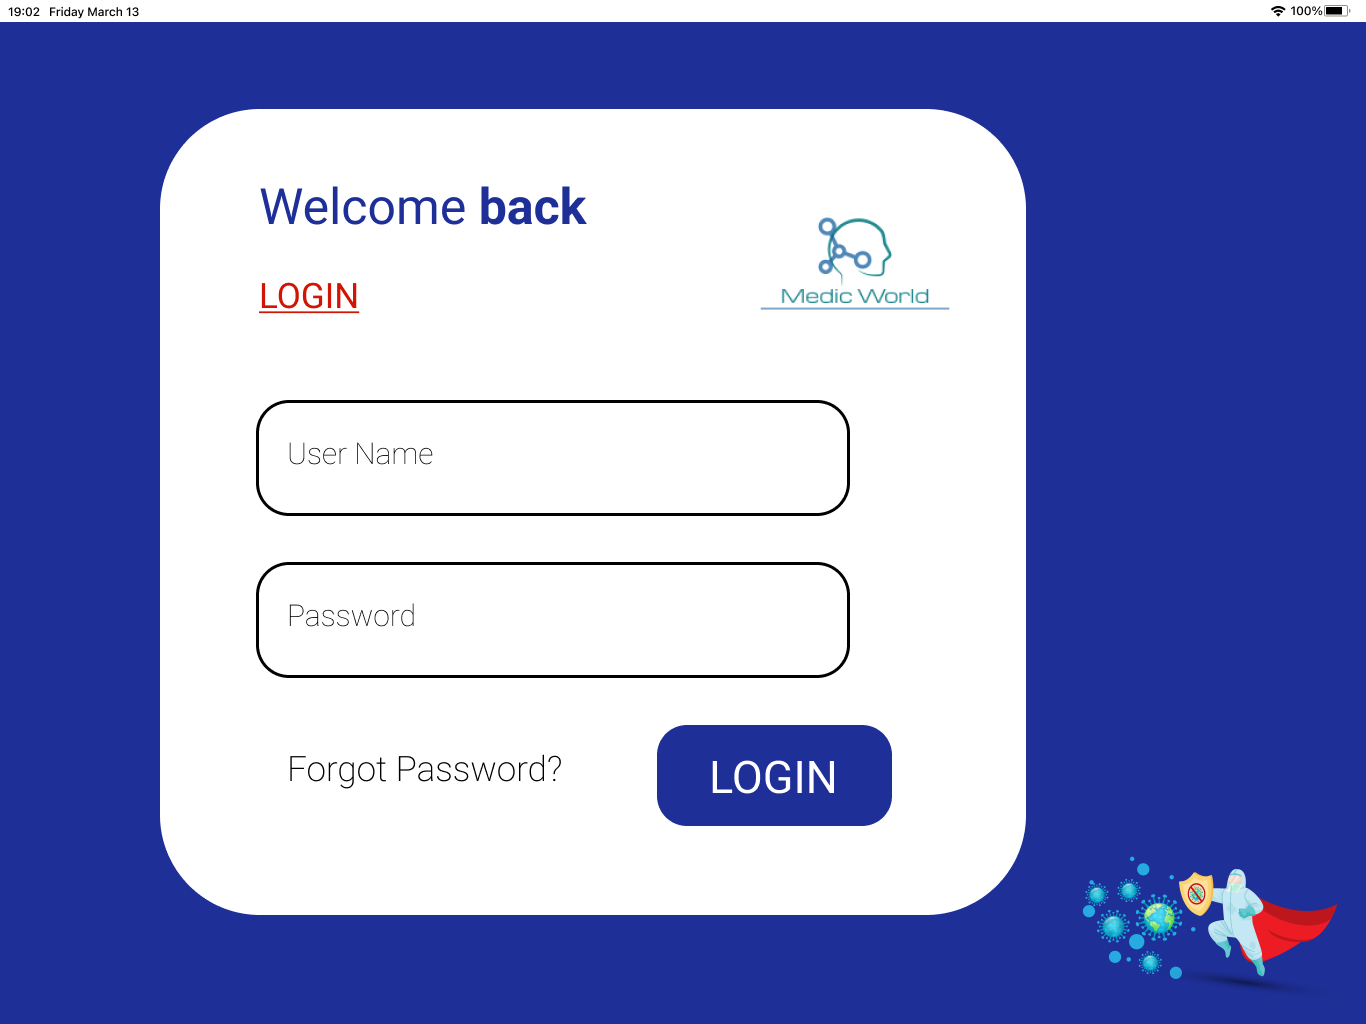
\includegraphics[width=0.5\textwidth]{Log in.png}
\caption{\label{fig:log in page} Οθόνη Εισόδου}
\end{figure}

\subsection{Κεντρική Σελίδα (Γιατρός)}

Σε περίπτωση που συνδεθεί στο \textbf{Medic World} με τους κωδικούς του ένας από του γιατρούς του προσωπικού, θα οδηγηθεί στην παρακάτω αρχική σελίδα (εικόνα 2). Κάποιες από τις λειτουργίες που προσφέρει η συγκεκριμένη οθόνη, είναι οι εξής:

\begin{itemize}
  \item Εμφανίζεται το πρόγραμμα που έχει ο γιατρός μέσα στην μέρα
  \item Πρόσφατες ενημερώσεις που αφορούν το νοσκομείο και την διαχείριση των ασθενών, ώστε να έχει πλήρη ενημέρωση
\end{itemize}

\vspace{0.3cm}

\begin{figure}[!htb]
\centering
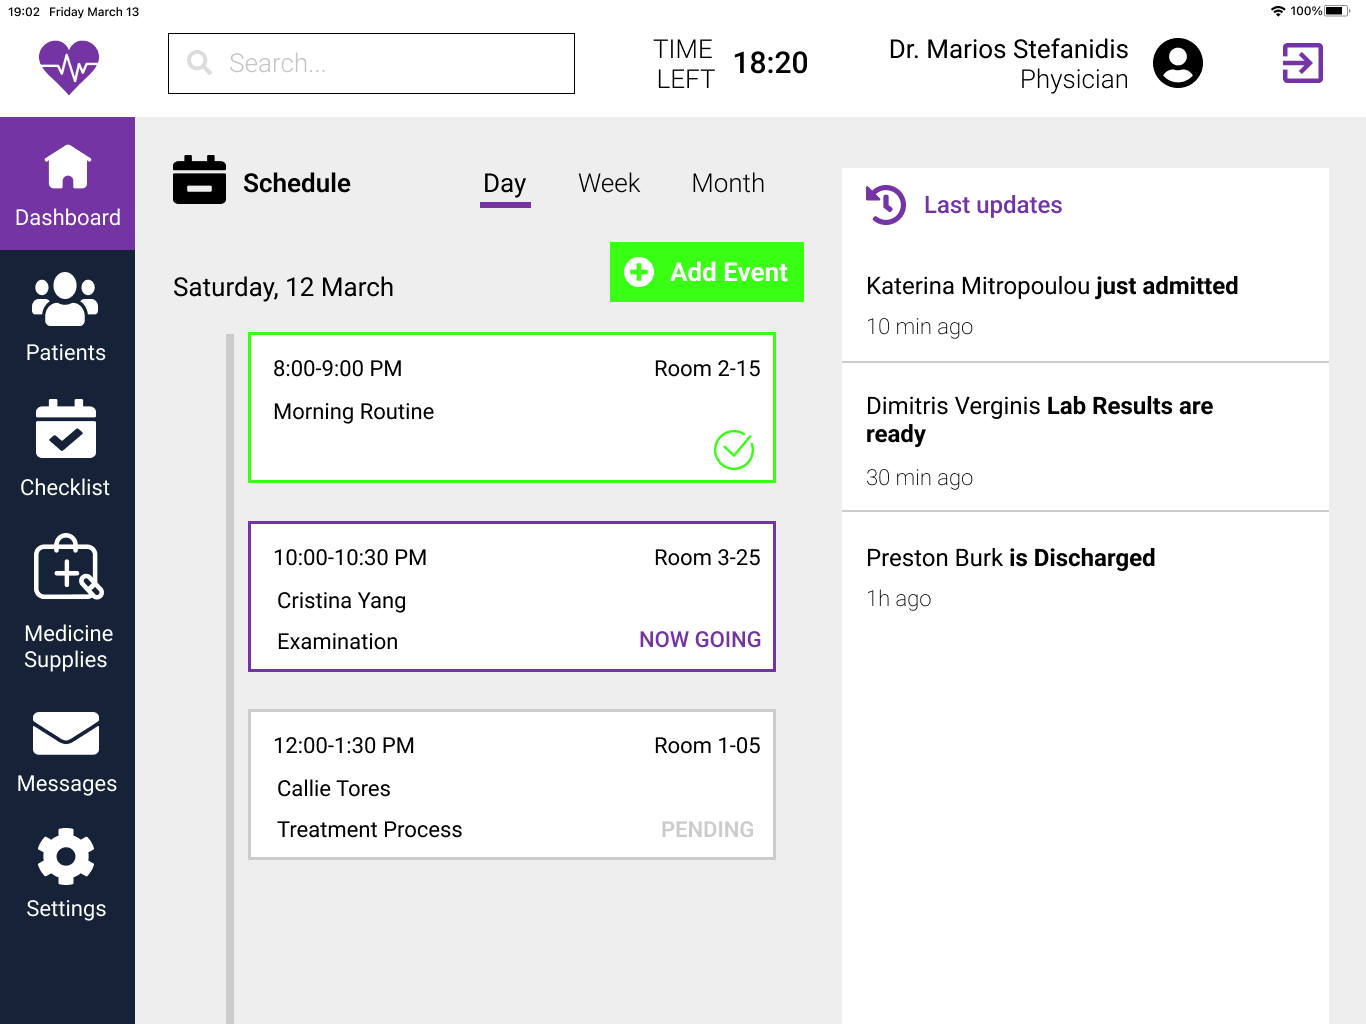
\includegraphics[width=0.5\textwidth]{Main Page (Doctor).png}
\caption{\label{fig:main page} Κεντρική Σελίδα Γιατρού}
\end{figure}


\subsection{Καρτέλες Ασθενών}

Επιλέγοντας τη λειτουργία patients ο χρήστης οδηγείται σε μία λίστα αποτελούμενη από τις καρτέλες των ασθενών (εικόνα 3). Κάθε καρτέλα περιλαμβάνει βασικές ενδείξεις που χρειάζεται να γνωρίζει ο γιατρός. \par
Η κεντρική ιδεά είναι να εμφανιζόνται οι ζωτικές ενδείξεις των ασθενών που γίνονται monitoring απευθείας στην εφαρμογή. Σε περίπτωση εμφάνισης κάποιας ακραίας τιμής (είτε προς τα κάτω, είτε προς τα πάνω), θα εμφανίζεται αμέσως ειδοποίηση στον γιατρό, ενώ η τιμή κάθε ζωτικής ένδειξης θα συνοδεύεται με το αντίστοιχο χρώμα λαμβάνοντας υπόψιν το κίνδυνο που διατρέχει ο ασθενής (πράσινο - φυσιολογική, κόκκινο - κίνδυνος, πορτοκαλί - προσοχή).

\vspace{0.3cm}

\begin{figure}[!htb]
\centering
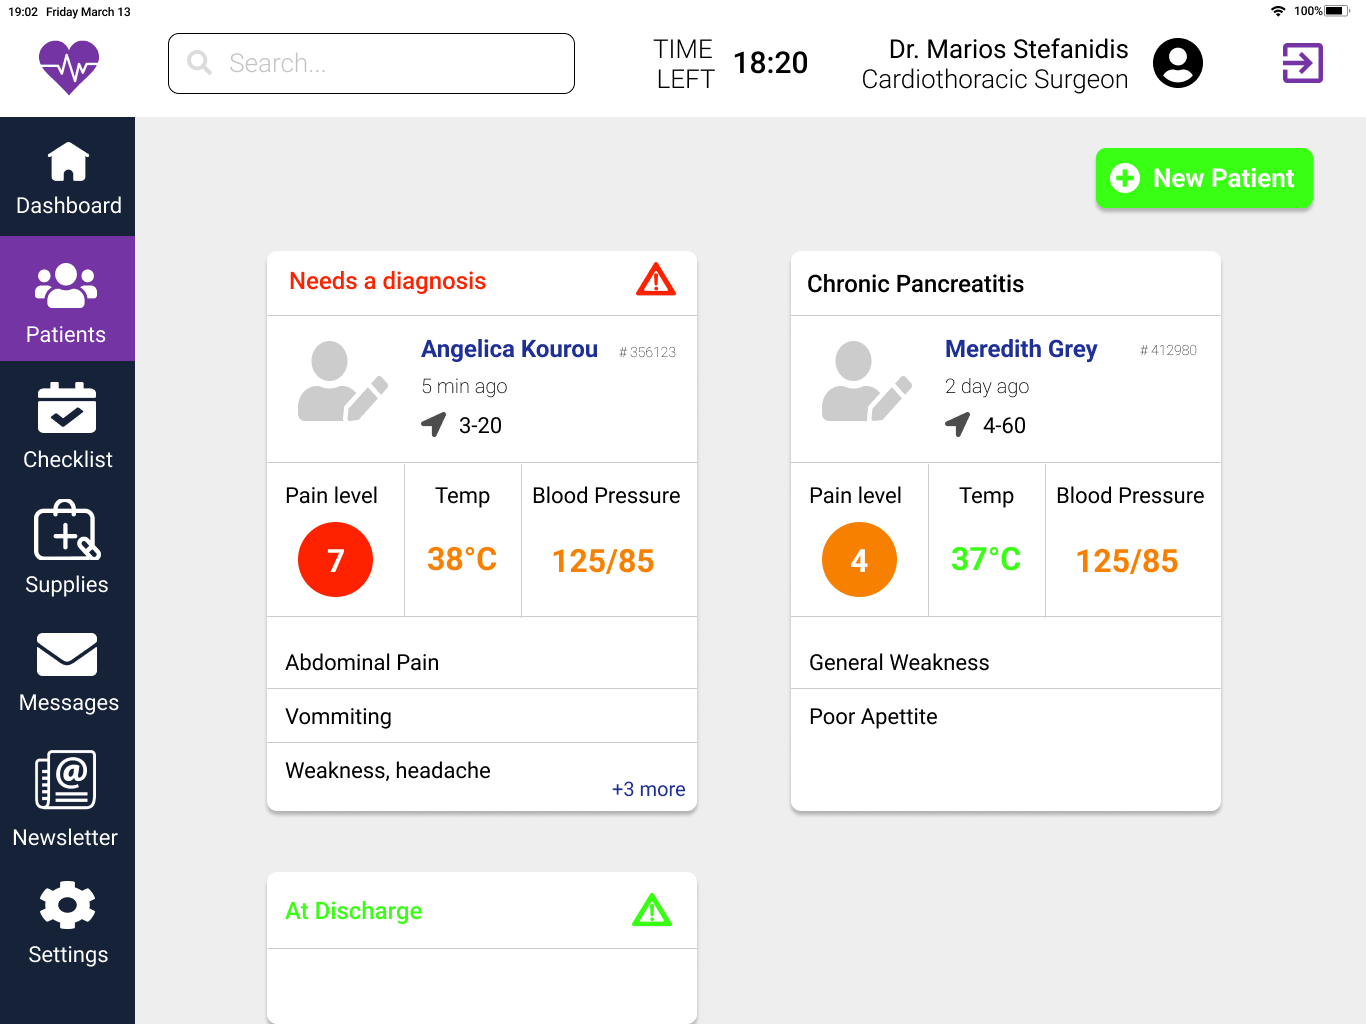
\includegraphics[width=0.5\textwidth]{Patients.png}
\caption{\label{fig:patients cards} Καρτέλες Ασθενών}
\end{figure}

\subsection{Προφίλ Ασθενών}

Πατώντας πάνω στο όνομα ενός ασθενούς στην εικόνα 3, εμφανίζεται η εικόνα 4, η οποία περιέχει περισσότερες λεπτομέρειες και σημαντικές πληροφορίες που αφορούν τον συγκεκριμένο ασθενή, όπως είναι η εμφάνιση των εργαστηριακών αποτελεσμάτων (εικόνα 5), οι οποίες θα εισάγονται στο σύστημα αμέσως μόλις πραγματοποιηθούν. \par
Μπορεί ακόμα να πραγματοποιηθεί προσθήκη νέων συμπτωμάτων και ιστορικού με τη χρήση του πληκτρολογίου ή της φωνητικής αναζήτησης. Επίσης, ο γιατρός μπορεί να προσθέσει επιπλέον εξετάσεις (Diagnostic Workup), στις οποίες θα του εμφανίζονται κάποιες προτεινόμενες, σύμφωνα με την αρχική διάγνωση που έχει γίνει, ώστε τελικά να πραγματοποιεί την τελική διάγνωση.
Θα μπορεί να καταγράφεται με λεπτομερή τρόπο το πλάνο φροντίδας του ασθενούς (care plan, εικόνα 6), όπως είναι η διατροφή, οι δοσοληψίες φαρμάκων, τα χειρουργία που πρέπει να γίνουν ή έγιναν και να διατηρείται ένα ιστορικό (patient profile, εικόνα 7) που θα περιλαμβάνει τα δημογραφικά και κλινικά δεδομένα του, ενώ ακόμη μέσω της συγκεκριμένης καρτέλας ο γιατρός θα έχει τη δυνατότητα να δώσει εξιτήριο στον εκάστοτε ασθενή.

\begin{figure}[!htb]
\centering
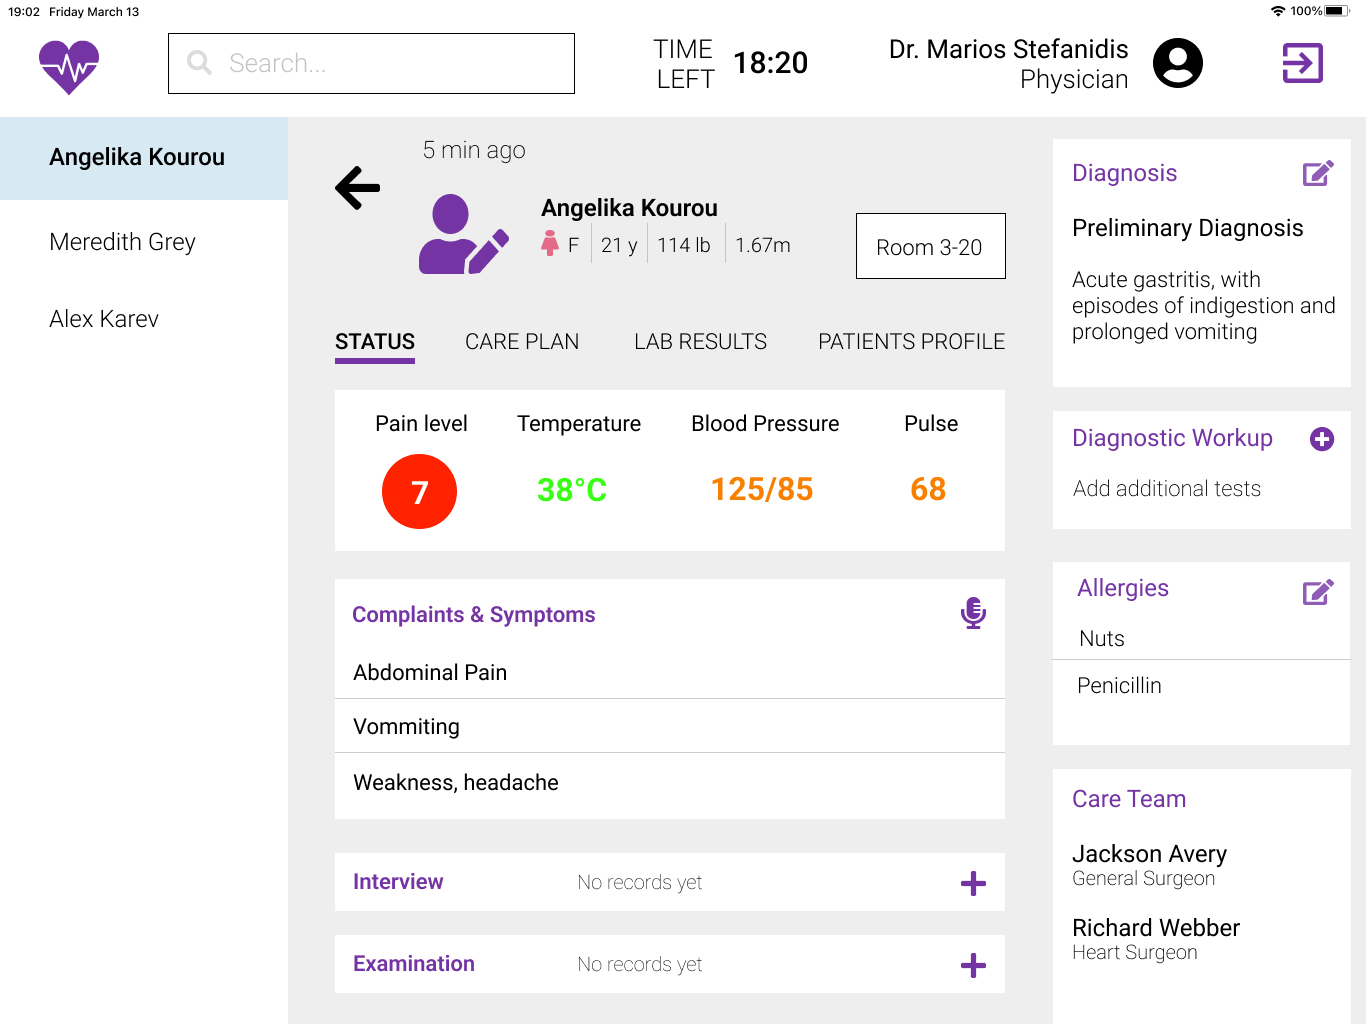
\includegraphics[width=0.5\textwidth]{Patients Cards (Status).png}
\caption{\label{fig:patient profile} Κατάσταση Ασθενούς}
\end{figure}

\newpage

\begin{figure}[!htb]
\centering
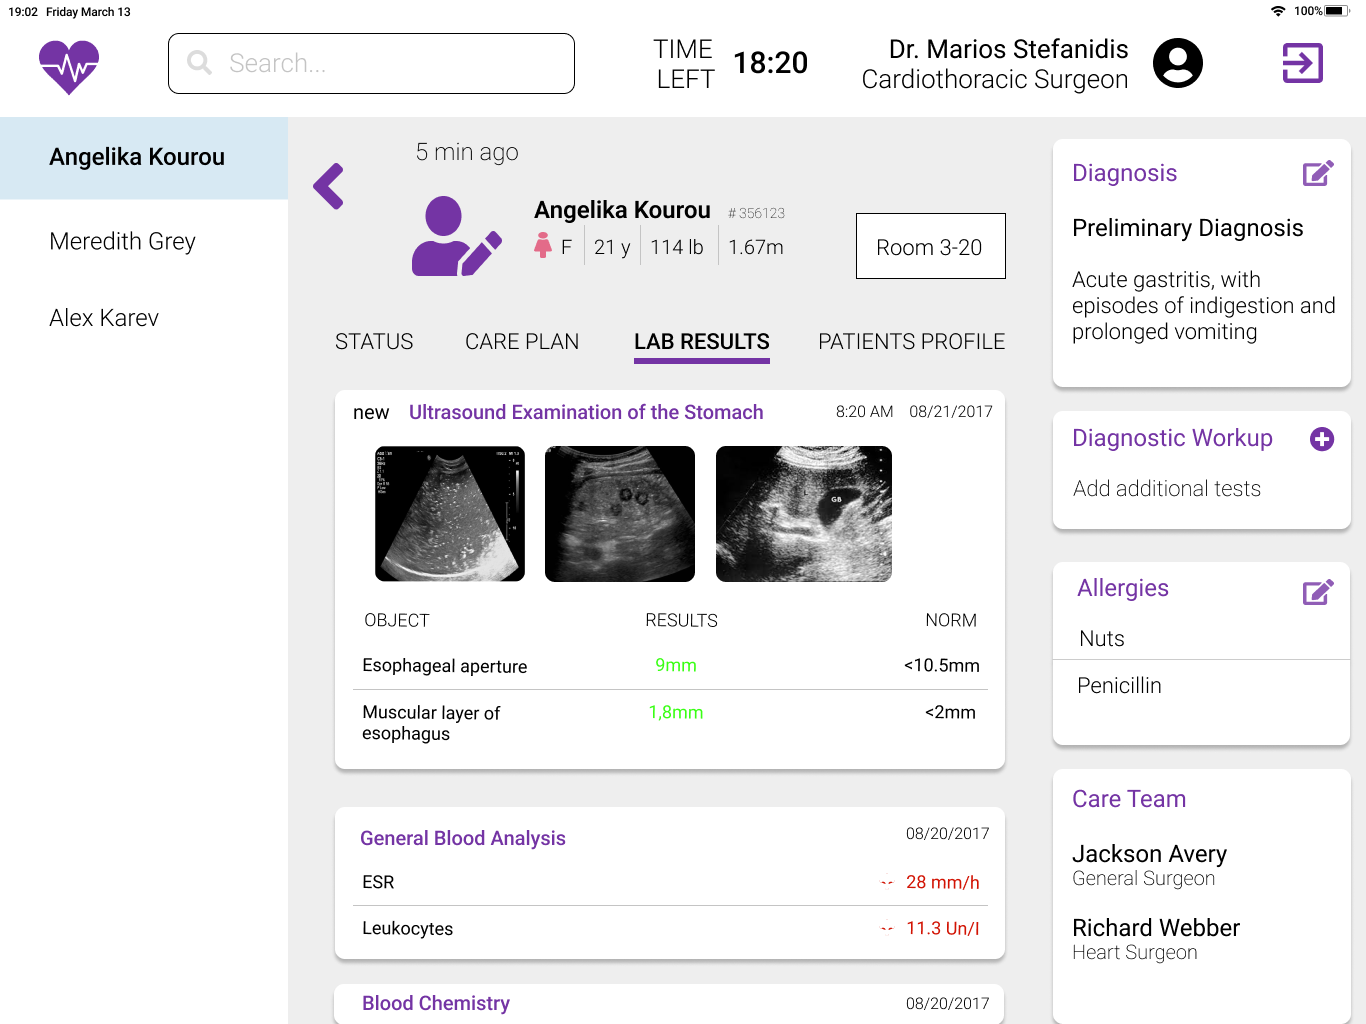
\includegraphics[width=0.5\textwidth]{Patients Cards (Lab Results).png}
\caption{\label{fig:Lab Results} Αποτελέσματα Εξετάσεων Ασθενούς}
\end{figure}

\begin{figure}[!htb]
\centering
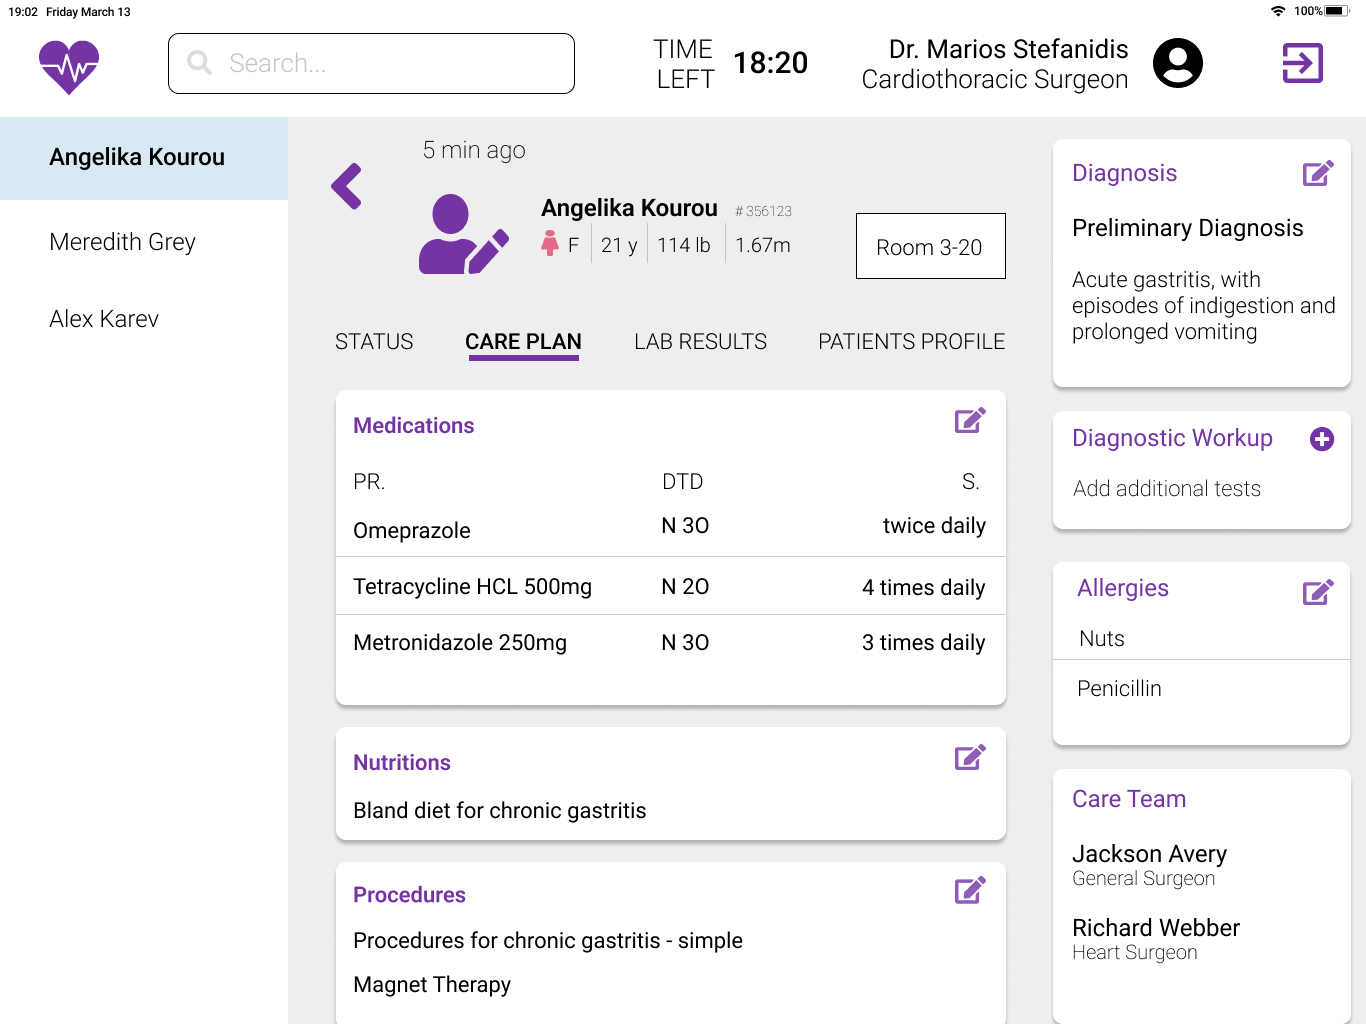
\includegraphics[width=0.5\textwidth]{Patients Cards (Care Plan).png}
\caption{\label{fig:Care Plan} Πρόγραμμα Περίθαλψης}
\end{figure}

\vspace{0.3cm}

\begin{figure}[!htb]
\centering
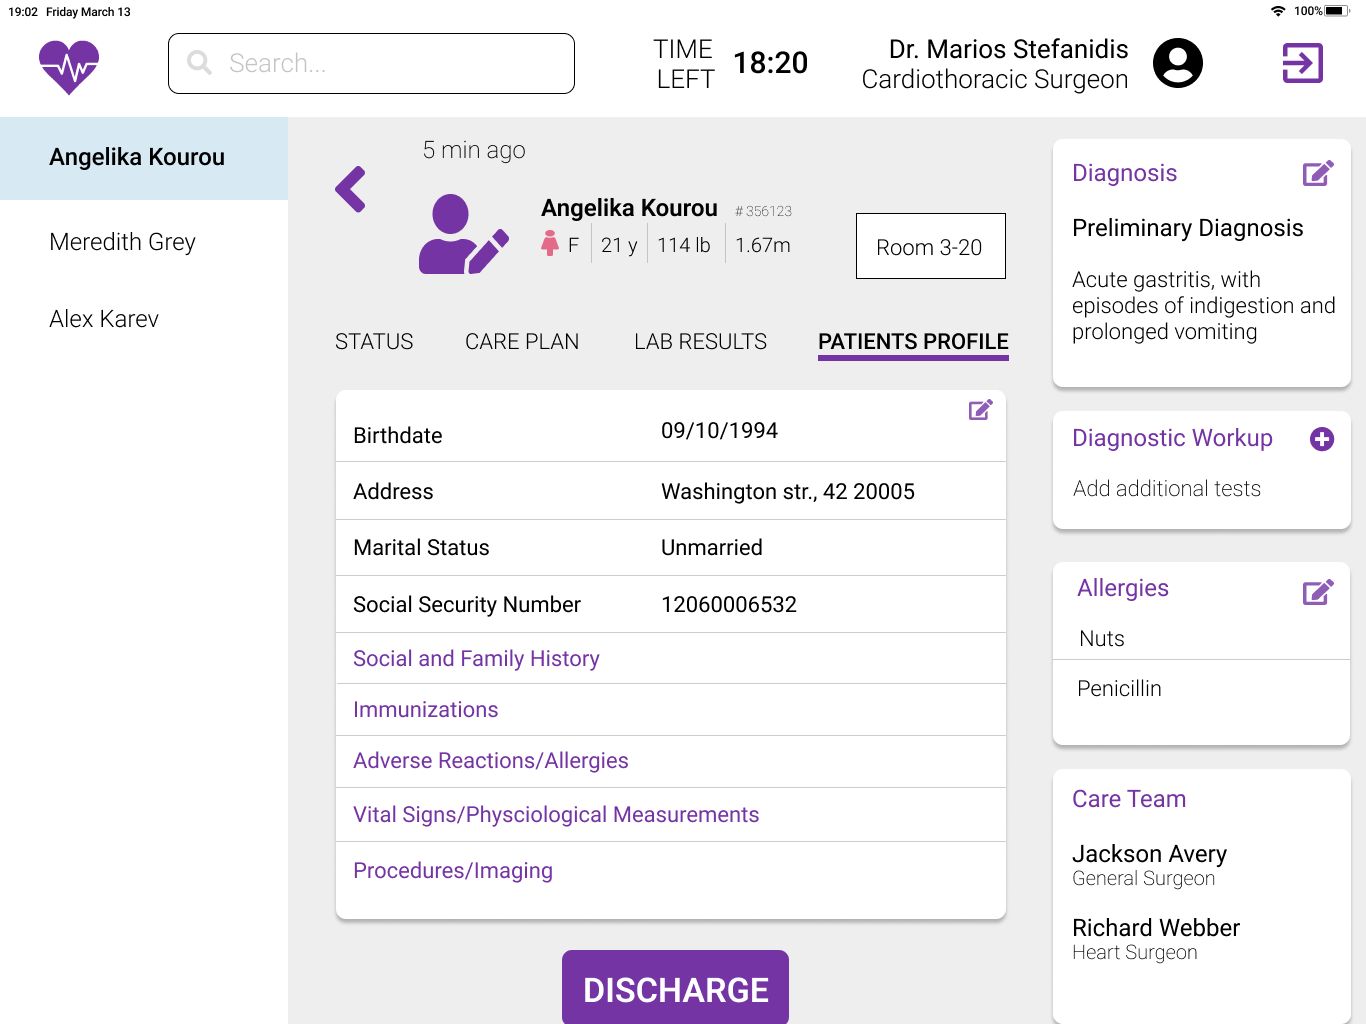
\includegraphics[width=0.5\textwidth]{Patients Cards (Patient's Profile).png}
\caption{\label{fig:Discharge} Προφίλ Ασθενούς - Έκδοση Εξιτηρίου}
\end{figure}

\newpage

\par Ακόμα, επιλέγοντας το Diagnostic Workup θα εμφανίζεται στα αριστερά της οθόνης ένα pop-window, το οποίο θα περιέχει πιθανές εξετάσεις που μπορεί να αναθέσει ο γιατρός στον ασθενή.

\begin{figure}[!htb]
\centering
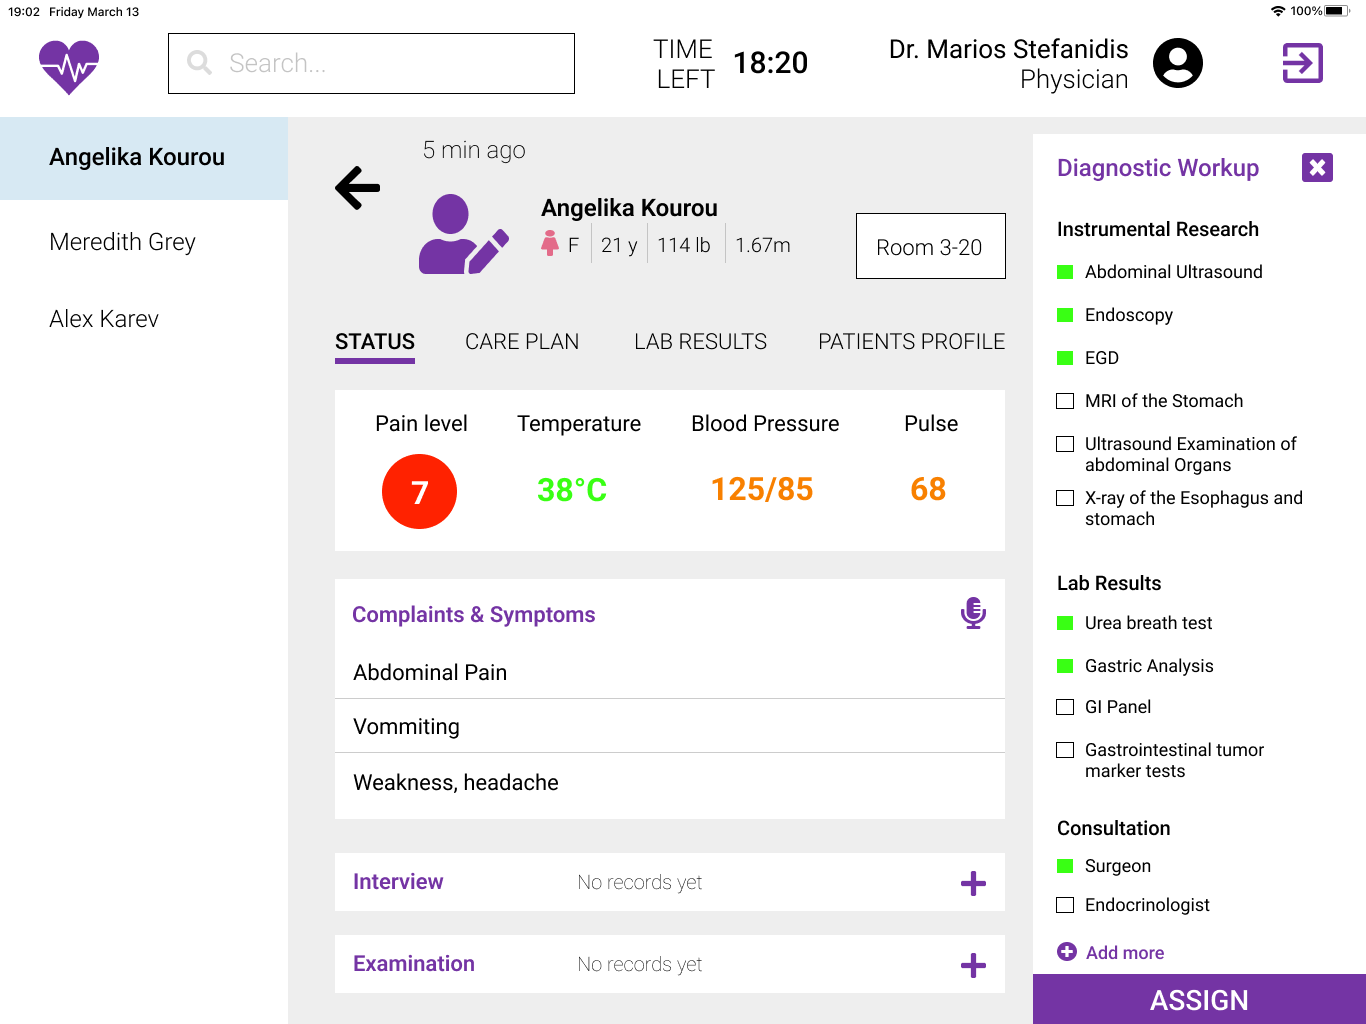
\includegraphics[width=0.5\textwidth]{Patients Cards (Status) (Diagnostic Workup).png}
\caption{\label{fig:Diagnostic Workup} Ανάθεση πιθανών Εξετάσεων }
\end{figure}

\vspace{0.3cm}

Τέλος, επιλέγοντας το Diagnosis θα εμφανίζεται στον γιατρό έναν "παράθυρο", στο οποίο θα μπορεί να προσθέσει την διάγνωση του ασθενούς με την βοήθεια του ICD-10 code (όπως αναφέρθηκε και παραπάνω) καθώς και της φωνητικής αναζήτησης.

\vspace{0.3cm}

\begin{figure}[!htb]
\centering
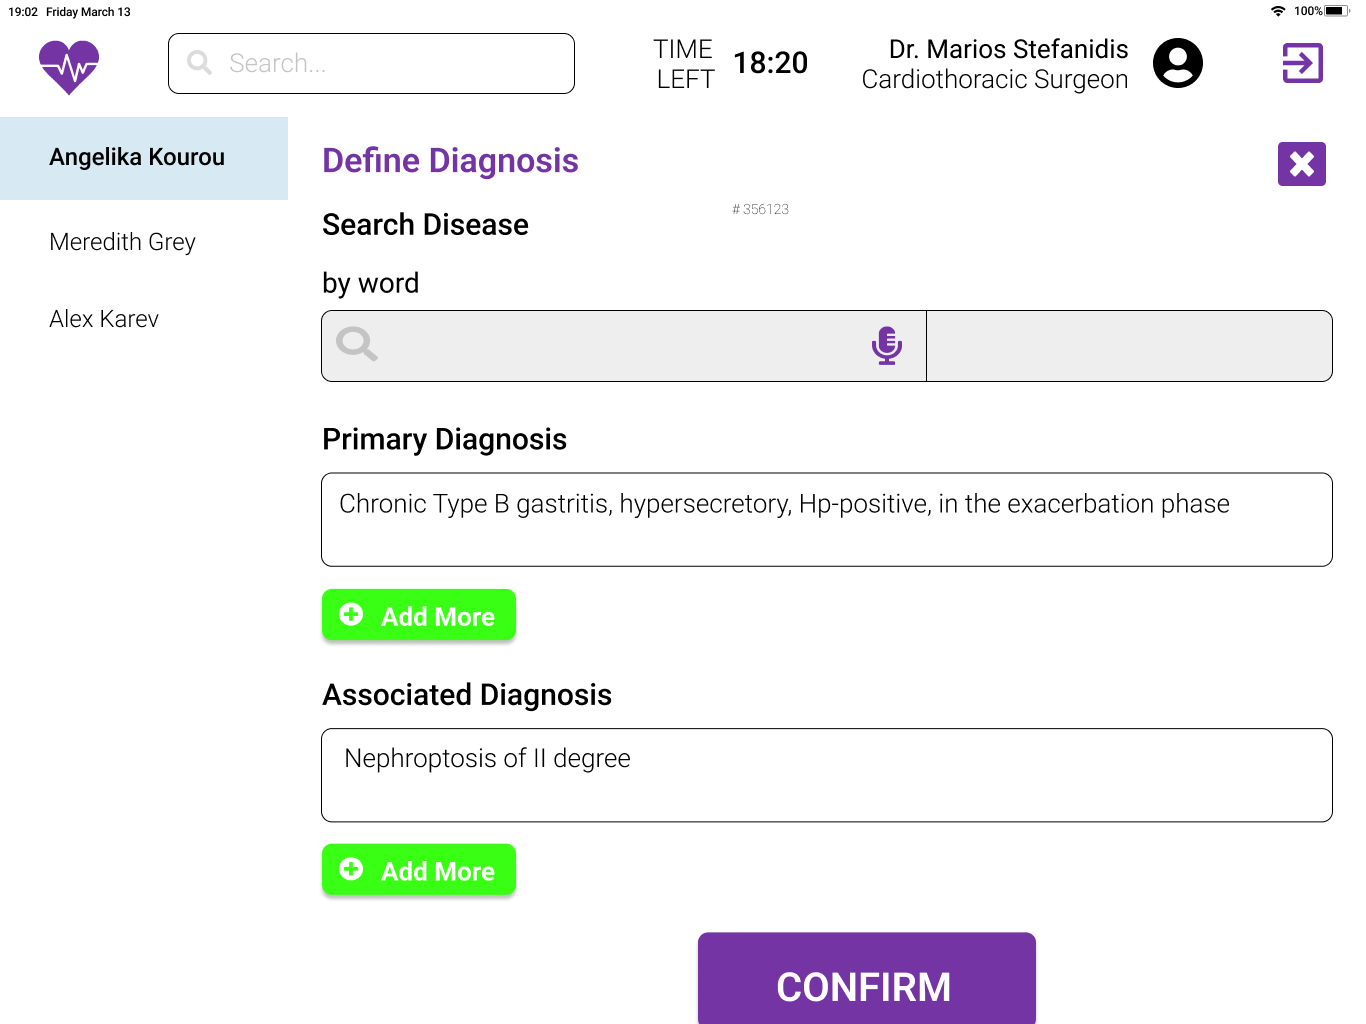
\includegraphics[width=0.5\textwidth]{Patients Cards (Status) (2).png}
\caption{\label{fig:Diagnosis} Διάγνωση Ασθενούς }
\end{figure}

\newpage

\subsection{Κατευθυντήριες Οδηγίες κατά την Έκδοση Εξιτηρίου}
(*) Κατά την έκδοση εξιτηρίου εμφανίζεται μία καρτέλα με τις οδηγίες του θεράποντος ιατρού που αφορούν τον ασθενή, την οποία μπορεί είτε να την κοινοποιήσει μέσω ηλεκτρονικού ταχυδρομείου είτε να την εκτυπώσει.

\begin{figure}[!htb]
\centering
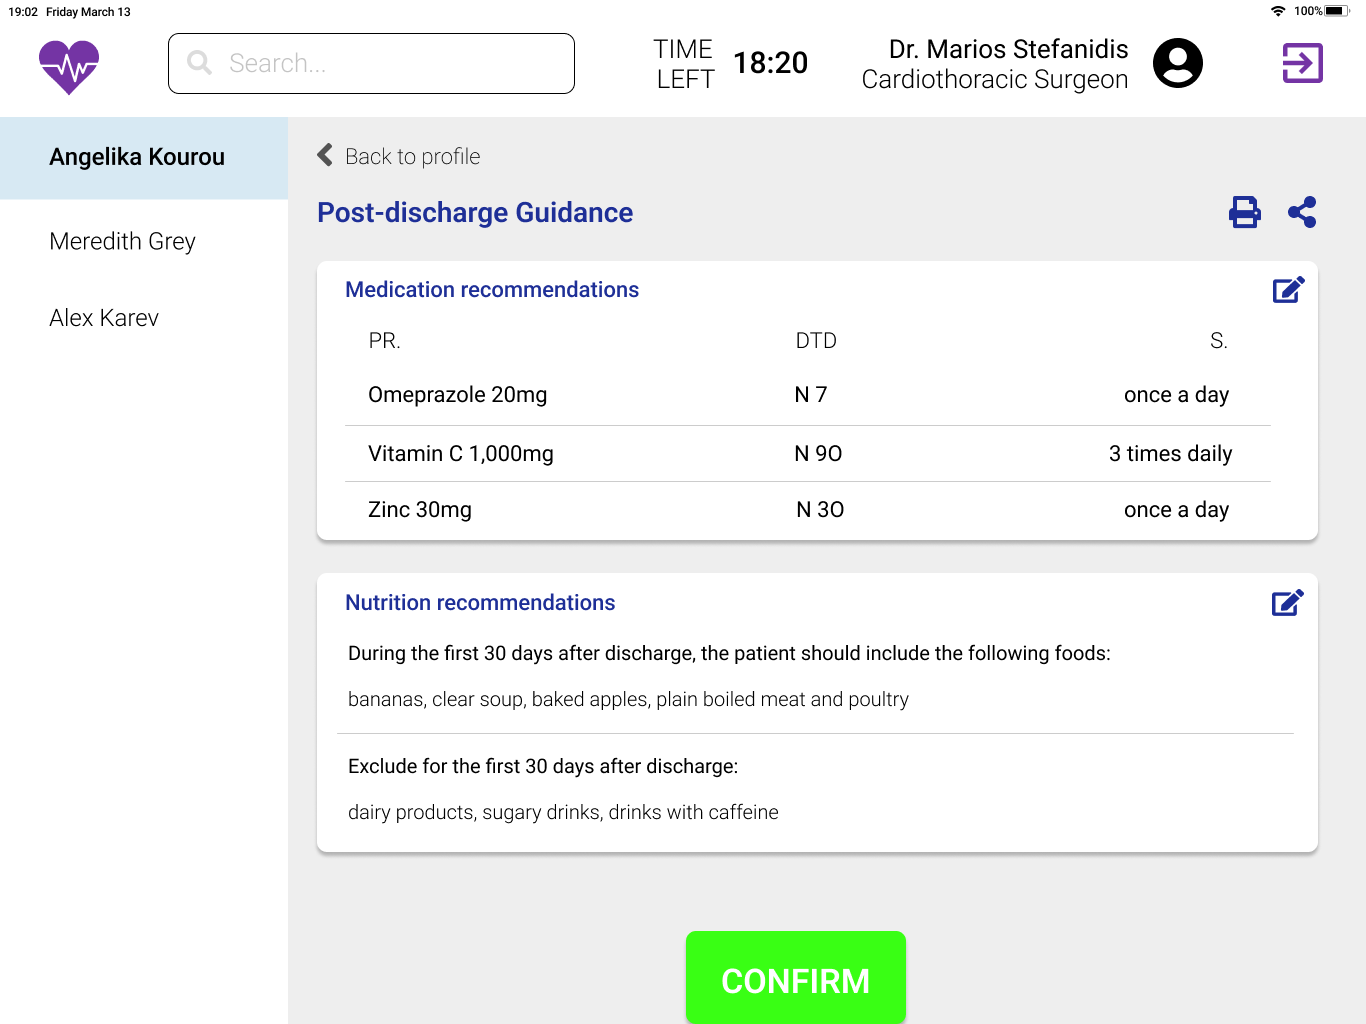
\includegraphics[width=0.5\textwidth]{Post-discharge Guidance.png}
\caption{\label{fig:discharge guide} Οδηγίες Εξιτηρίου}
\end{figure}

\subsection{Καταχώρηση Νέου Ασθενούς}
(*) Μέσω του \textbf{Medic World} στο ιατρικό και νοσηλευτικό προσωπικό δίνεται η δυνατότητα για καταχώρηση νέων ασθενών. Από το μενού των καρτελών των ασθενών (εικόνα 3) ο χρήστης επιλέγοντας τη λειτουργία "New Patient" εισέρχεται σε μία διαδικασία προσθήκης νέου ασθενούς. Αρχικά, στην οθόνη του εμφανίζεται (εικόνα 11) μία καρτέλα για τη συμπλήρωση των βασικών στοιχείων του ασθενούς (λ.χ. όνομα, ηλικία), ενώ στη συνέχεια όταν πλέον έχει δημιουργηθεί το νέο προφίλ, ο χρήστης καλείται να συμπληρώσει μία λεπτομερή φόρμα με όλες τις πληροφορίες που διατίθενται σχετικά με τον συγκεκριμένο ασθενή (εικόνα 12). 

\vspace{0.3cm}

\begin{figure}[!htb]
\centering
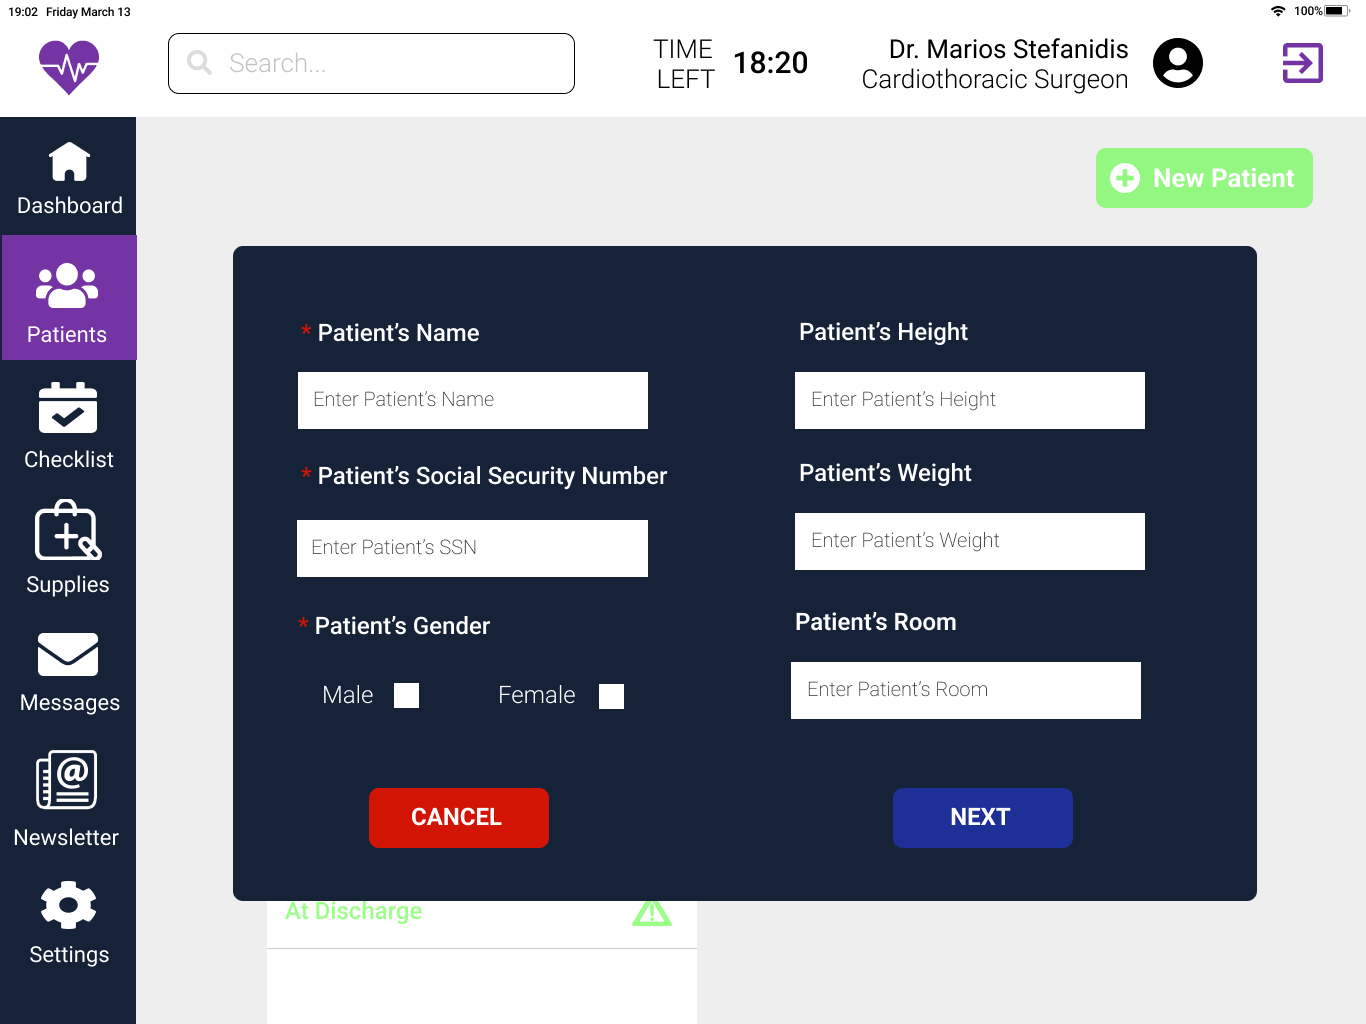
\includegraphics[width=0.5\textwidth]{New Patient.png}
\caption{\label{fig:new patient} Στοιχεία Νέου Ασθενούς }
\end{figure}

\newpage

\begin{figure}[!htb]
\centering
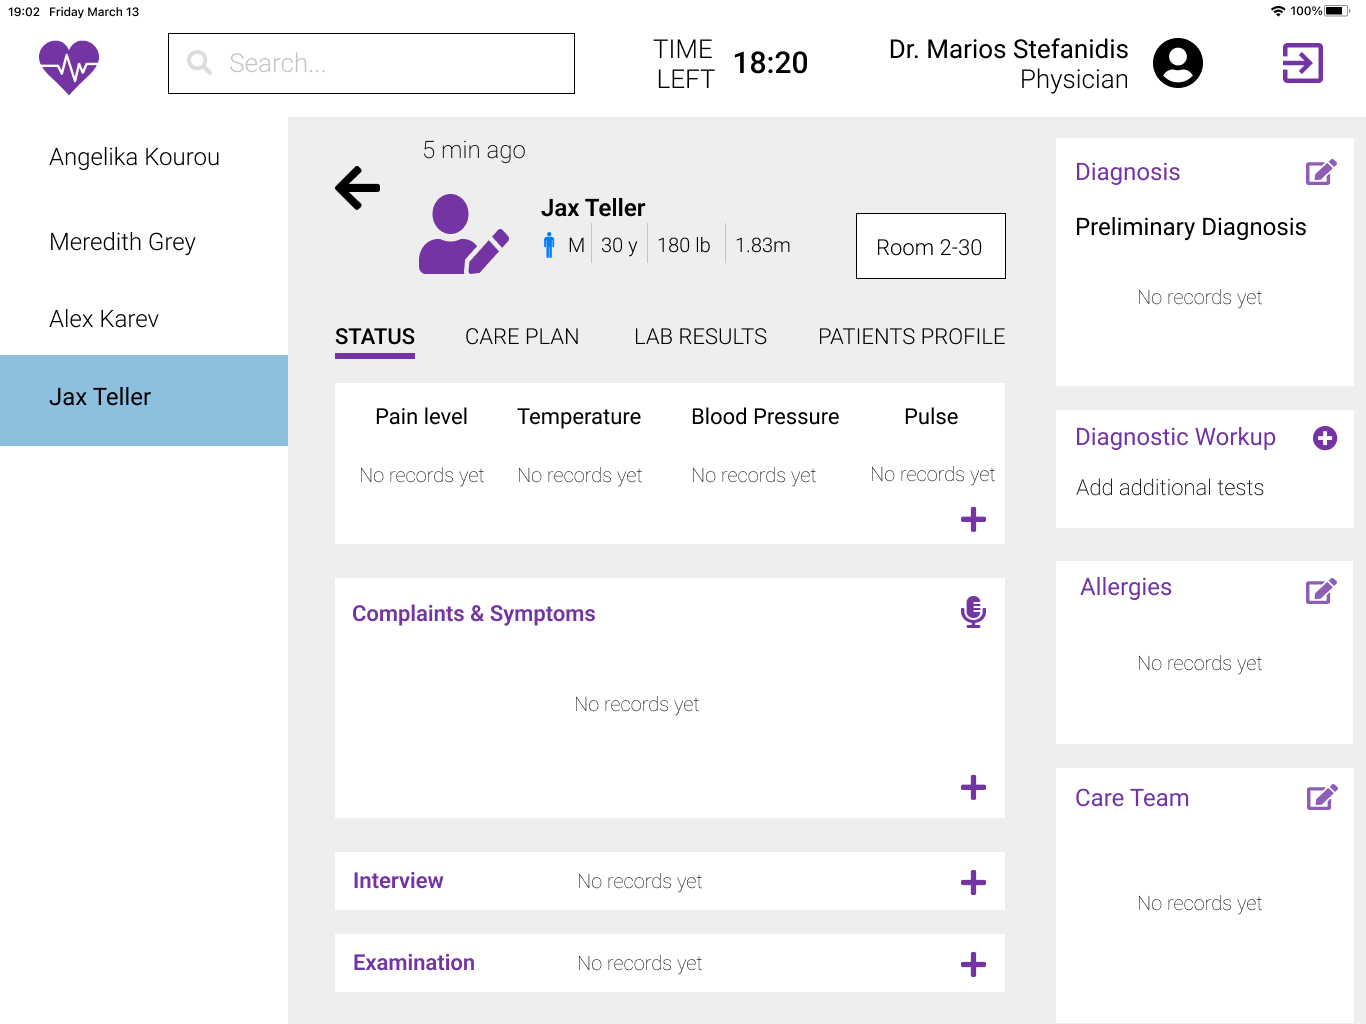
\includegraphics[width=0.5\textwidth]{New Patient Form.png}
\caption{\label{fig:new patient form} Αναλυτική Φόρμα Νέου Ασθενούς}
\end{figure}

\subsection{Λίστα Ελέγχου}

(*) Μία από τις λειτουργίες που προσφέρει το \textbf{Medic World} είναι ο εκάστοτε χρήστης ανά πάσα στιγμή να είναι σε θέση επιλέγοντας τη λειτουργία checklist να έχει πρόσβαση σε μία αρχική καρτέλα που παρουσιάζει πόσες κλίνες, χειρουργεία και εργαστήρια (πχ ακτινολογικό) είναι διαθέσιμα εκείνη τη στιγμή. Πατώντας στην κάθε κατηγορία θα εμφανίζονται τα εξής:

\begin{itemize}
  \item Laboratories: Τα εργαστήρια που είναι διαθέσιμα για παραγγελία εξετάσεων ή παραδείγματος χάριν οι αξονικοί τομογράφοι που είναι σε λειτουργία
  \item Operating Rooms: Τα χειρουργία που βρίσκονται σε εξέλιξη συνοδευόμενα από κάποιες σημαντικές πληροφορίες, όπως είναι ο γιατρός/οι γιατροί που χειρουργούν, ο ασθενής που χειρουργείται, η επέμβαση που πραγματοποιείται κλπ
  \item Rooms: τα δωμάτια και οι κλίνες που είναι διαθέσιμες
\end{itemize}

\vspace{0.3cm}

\begin{figure}[!htb]
\centering
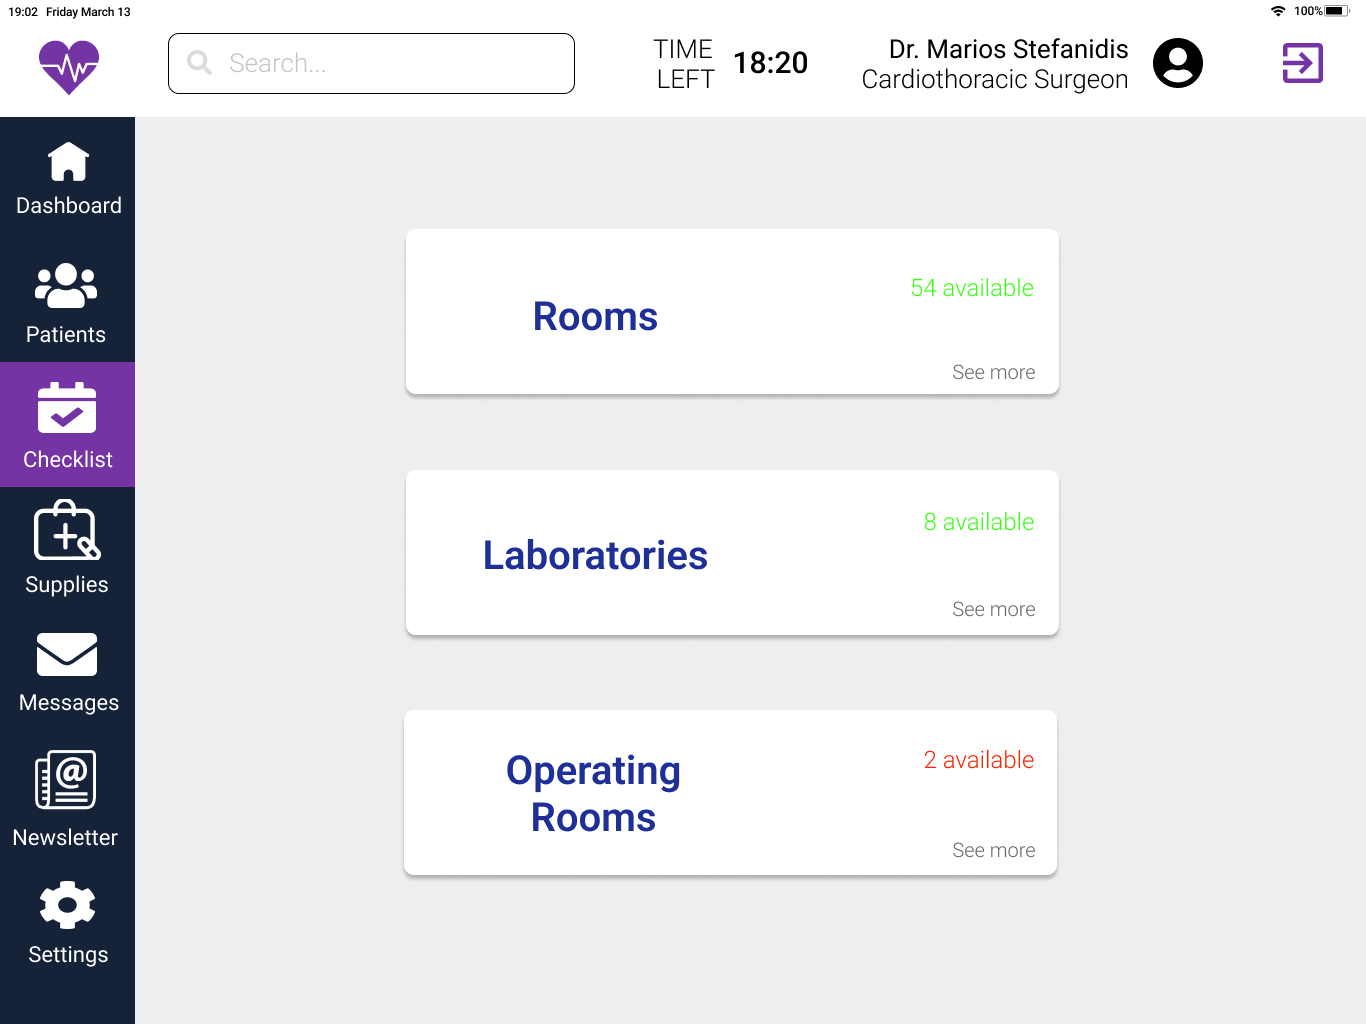
\includegraphics[width=0.5\textwidth]{Checklist.png}
\caption{\label{fig:checklist} Λίστα Ελέγχου}
\end{figure}

\subsubsection{Διαθεσιμότητα Δωματίων - Παράδειγμα Χειρουργείων}
(*) Όπως αναφέρθηκε ήδη το \textbf{Medic World} δίνει στο ιατρονοσηλευτικό προσωπικό τη δυνατότητα να ελέγχει ανά πάσα στιγμή τη διαθεσιμότητα της κλινικής σε δωμάτια, εργαστήρια καθώς και χειρουργεία. 
Eπιλέγοντας το κουμπί που αντιστοιχεί στα χειρουργεία (εικόνα 13) ο γιατρός ή ο νοσηλευτής οδηγείται σε μία καρτέλα που περιέχει όλα τα χειρουργικά δωμάτια (πρώτα με σειρά διαθεσιμότητας και έπειτα με αλφαβητική σειρά). Κατά αυτό τον τρόπο, δίνεται η δυνατότητα στο χρήστη επιλέγοντας κάποιο από τα κενά δωμάτια να δηλώσει στο σύστημα ότι πρόκειται να χρησιμοποιηθεί (εικόνα 15), ενώ επιλέγοντας κάποιο από τα μη διαθέσιμα δωμάτια καθίσταται εφικτό, ο γιατρός που είχε δηλωθεί ότι το χρησιμοποιούσε, να το δηλώσει ως διαθέσιμο όταν η εγχείρηση ολοκληρωθεί.

\vspace{0.3cm}

\begin{figure}[!htb]
\centering
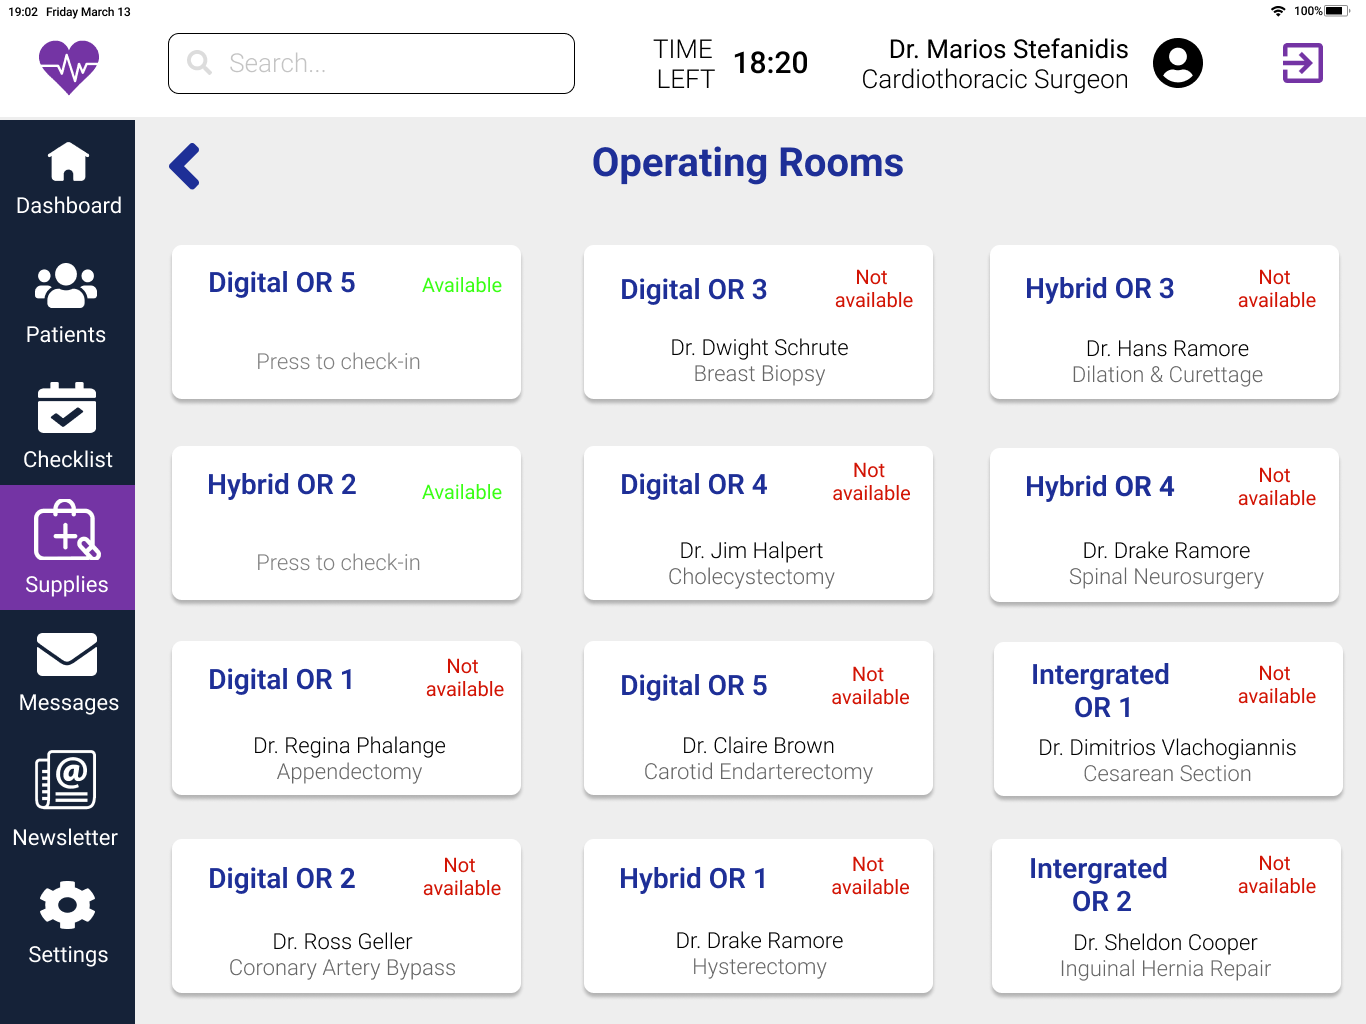
\includegraphics[width=0.5\textwidth]{Operating Rooms.png}
\caption{\label{fig:operating rooms} Λίστα Ελέγχου - Χειρουργεία}
\end{figure}

\vspace{0.3cm}

\begin{figure}[!htb]
\centering
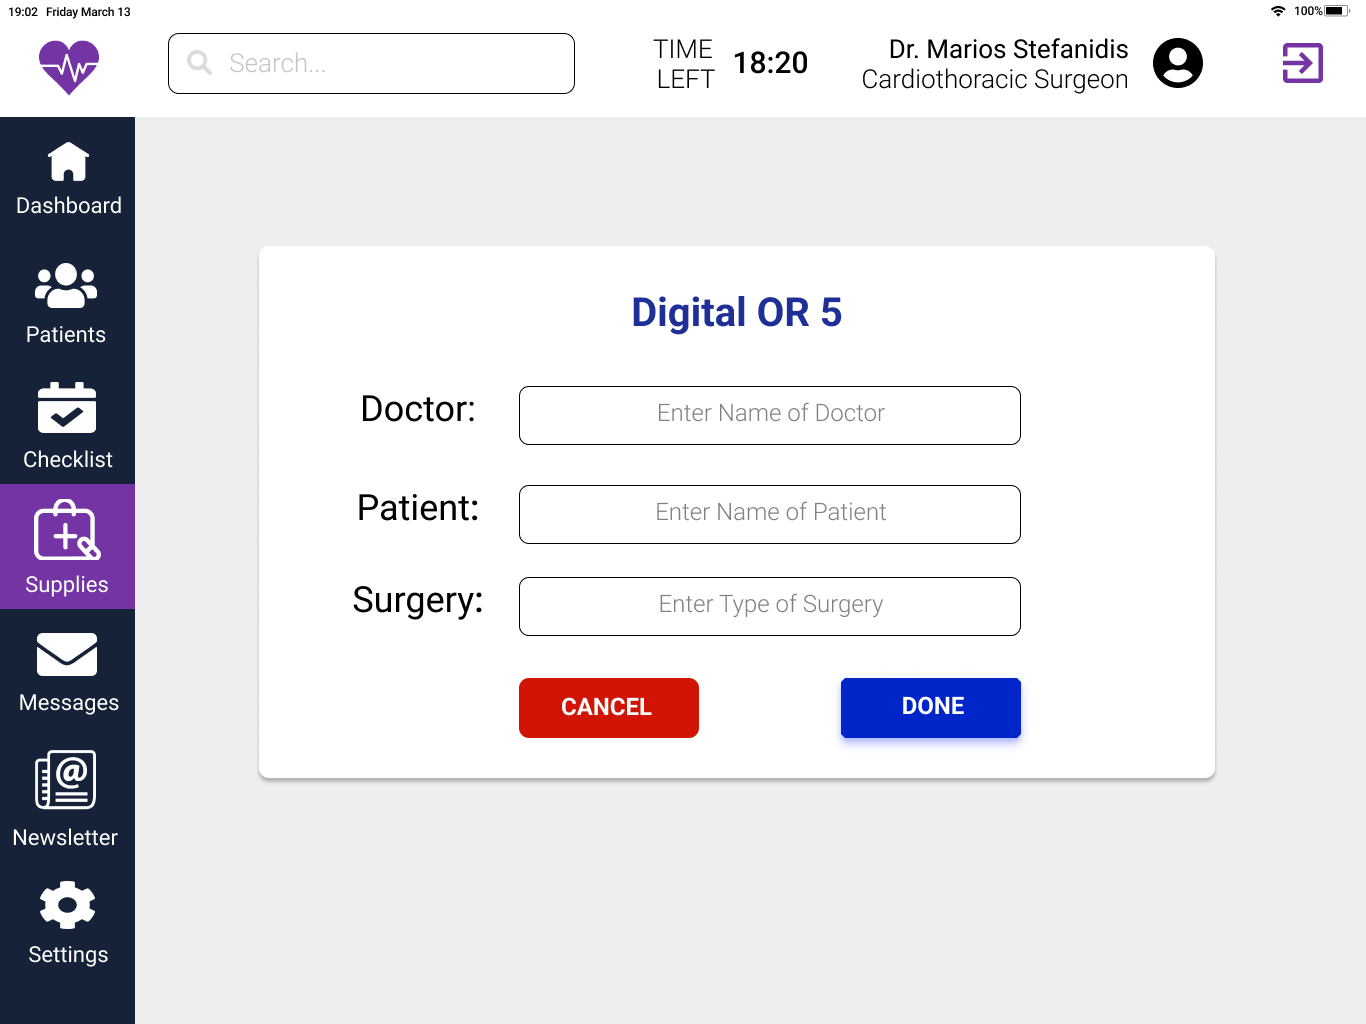
\includegraphics[width=0.5\textwidth]{OR Check-In.png}
\caption{\label{fig:OR availability} Δήλωση Απασχόλησης Χειρουργείου}
\end{figure}

\subsection{Φαρμακευτικές Προμήθειες}

(*) Τέλος, επιλέγοντας τη λειτουργία που αντιστοιχεί στις φαρμακευτικές προμήθειες ο χρήστης θα οδηγείται σε μία καρτέλα με τα περιεχόμενα της φαρμακαποθήκης.
Ανάλογα με την επαγγελματική του ιδιότητα στη συγκεκριμένη καρτέλα ο χρήστης έχει στη διάθεση του και διαφορετικές λειτουργίες. \par
Αν το κουμπί "Medicine Supplies" επιλεχθεί από έναν γιατρό/νοσηλευτή, τότε αυτός οδηγείται σε μία καρτέλα με κατηγορίες φαρμάκων και στη συνέχεια επιλέγοντας μία από τις κατηγορίες μπορεί να ελέγξει τη διαθεσιμότητα στο φάρμακο που επιθυμεί (εικόνα 16). Επιλέγοντας μια από τις κατηγορίες φαρμάκων. \par
Αν ο χρήστης ανήκει στο φαρμακευτικό προσωπικό του νοσοκομείου, τότε μέσω του "Medicine Supplies" οδηγείται στην ίδια καρτέλα με το γιατρό με τη διαφορά ότι τώρα δίνεται στο χρήστη μία επιλογή για προσθήκη νέου φαρμάκου (εικόνα 17). Στη συνέχεια, αν επιλεχθεί η συγκεκριμένη λειτουργία, τότε στην οθόνη εμφανίζεται μία φόρμα για τη δήλωση του νέου φαρμάκου (εικόνα 18). \par
Σημειώνεται ότι το φαρμακευτικό προσωπικό θεωρείται υπεύθυνο για τη διαχείριση της φαρμακαποθήκης και θα μπορεί προφανώς να εκτελεί παραγγελίες των φαρμάκων που βρίσκονται σε έλλειψη, ενώ θα μπορεί να υπάρξει και ένα system log, που θα καταγράφει τα φάρμακα που έχουν χρησιμοποιηθεί αλλά και τον λόγο χρήσης τους, προκειμένου να αποφευχθούν τυχόν παρανομίες.
Τέλος, επιλέγοντας μία από τις κατηγορίες των φαρμάκων (λ.χ. αντιβιοτικά, εικόνα 16) ο εκάστοτε οδηγείται σε μία καρτέλα που περιλαμβάνει όλα τα φάρμακα που ανήκουν στην συγκεκριμένη κατηγορία (εικόνα 19). \vspace{0.3cm}

\textbf{Σημείωση:} Στην εικόνα 17 παρατηρούμε τις διαφορετικές λειτουργίες που έχει ένας φαρμακοποιός από το μενού που βρίσκεται στο αριστερό πλαίσιο της εικόνας.

\vspace{0.3cm}

\begin{figure}[!htb]
\centering
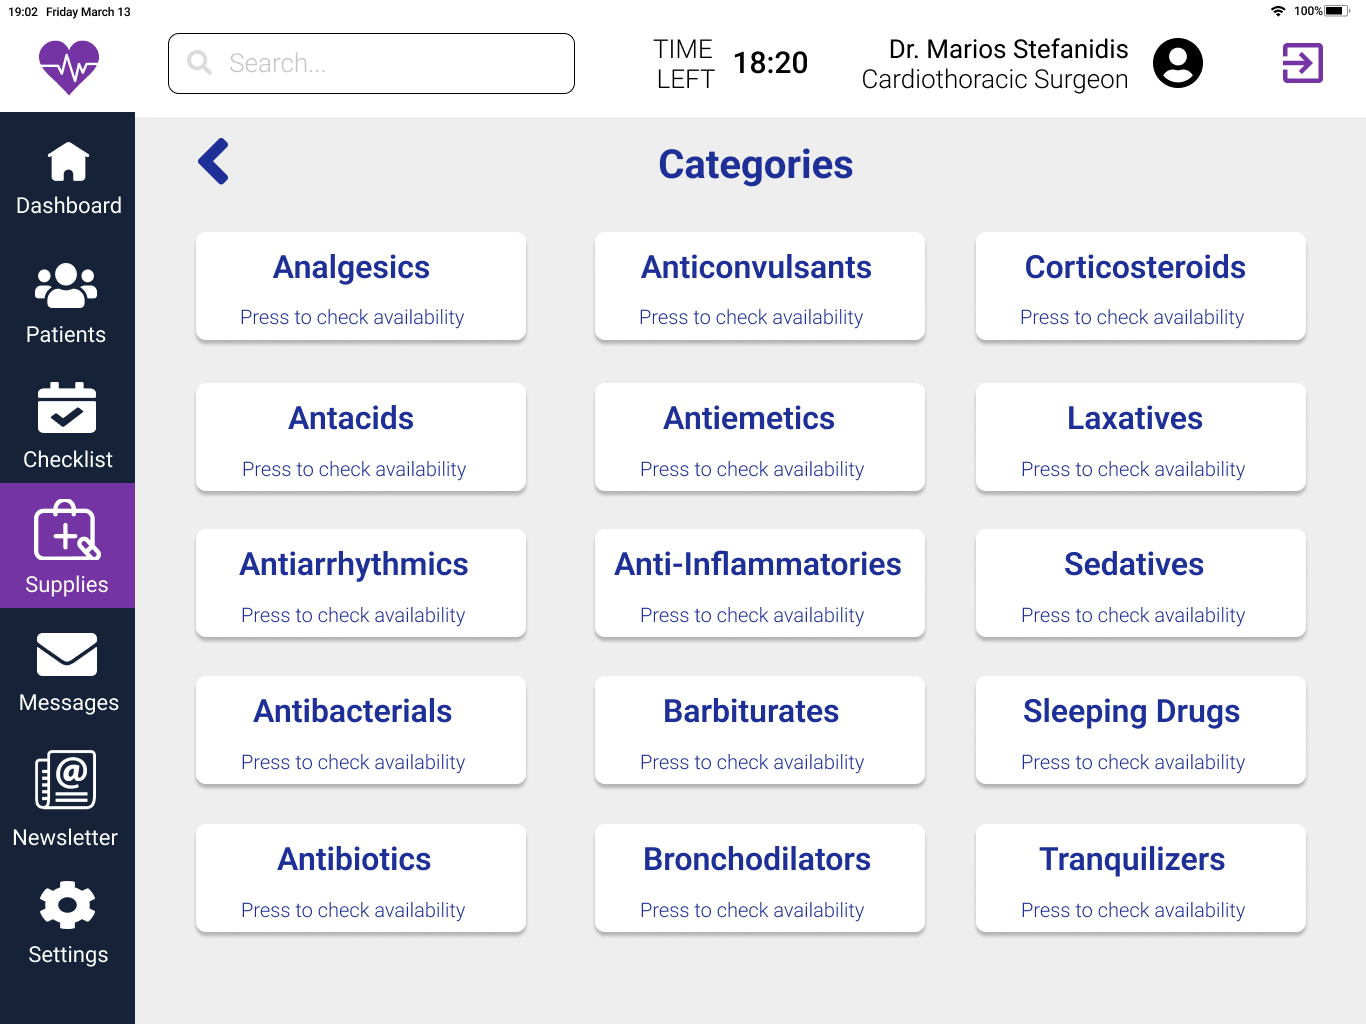
\includegraphics[width=0.5\textwidth]{Medicine Supplies Categories.png} 
\caption{\label{fig:doctor/nurse} Προμήθειες Φαρμάκων (Χρήστης Γιατρός/Νοσηλευτής)}
\end{figure}

\vspace{0.3cm}

\begin{figure}[!htb]
\centering
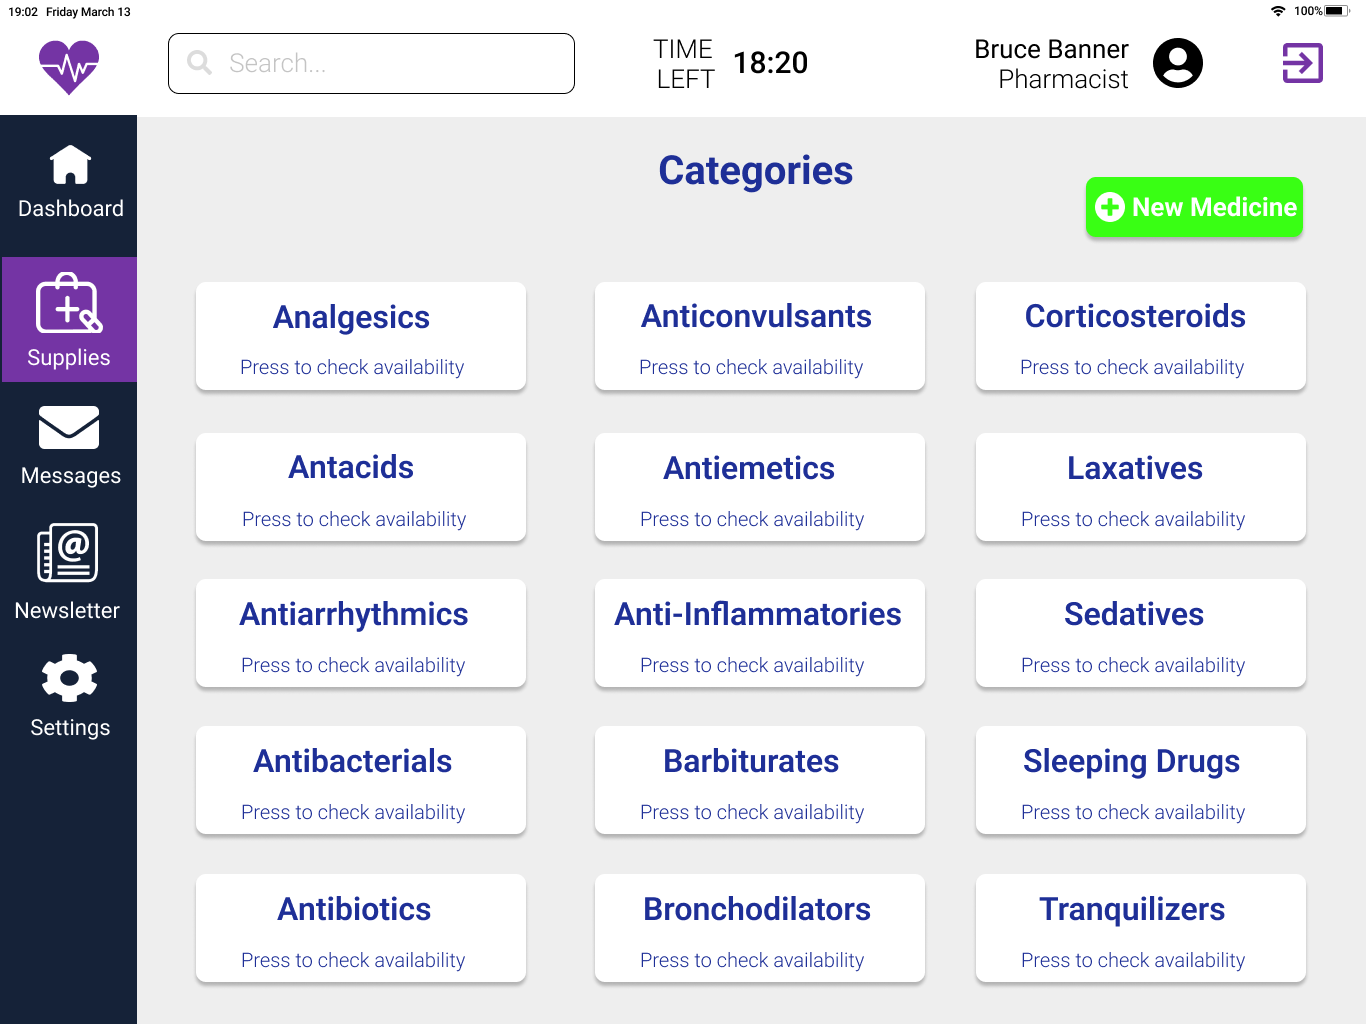
\includegraphics[width=0.5\textwidth]{Medicine Supplies Categories (Pharmacist).png} 
\caption{\label{fig:Medical Supplies} Προμήθειες Φαρμάκων (Χρήστης Φαρμακοποιός)}
\end{figure}

\newpage

\begin{figure}[!htb]
\centering
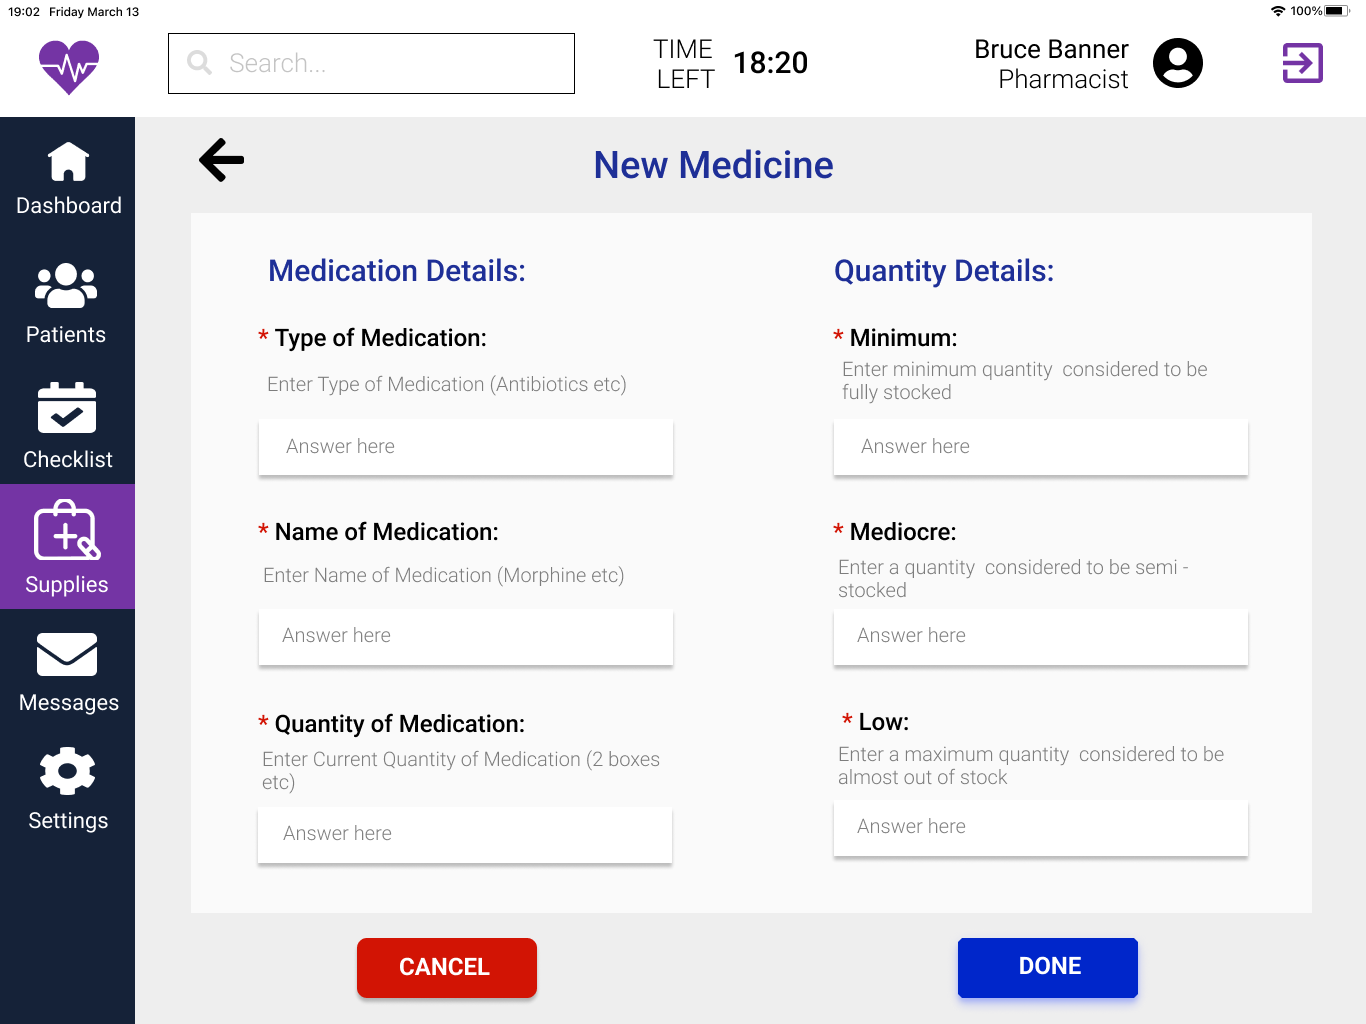
\includegraphics[width=0.5\textwidth]{New Medicine.png} 
\caption{\label{fig:new medicine} Καταχώρηση Νέου Φαρμάκου}
\end{figure}

\vspace{0.3cm}

\begin{figure}[!htb]
\centering
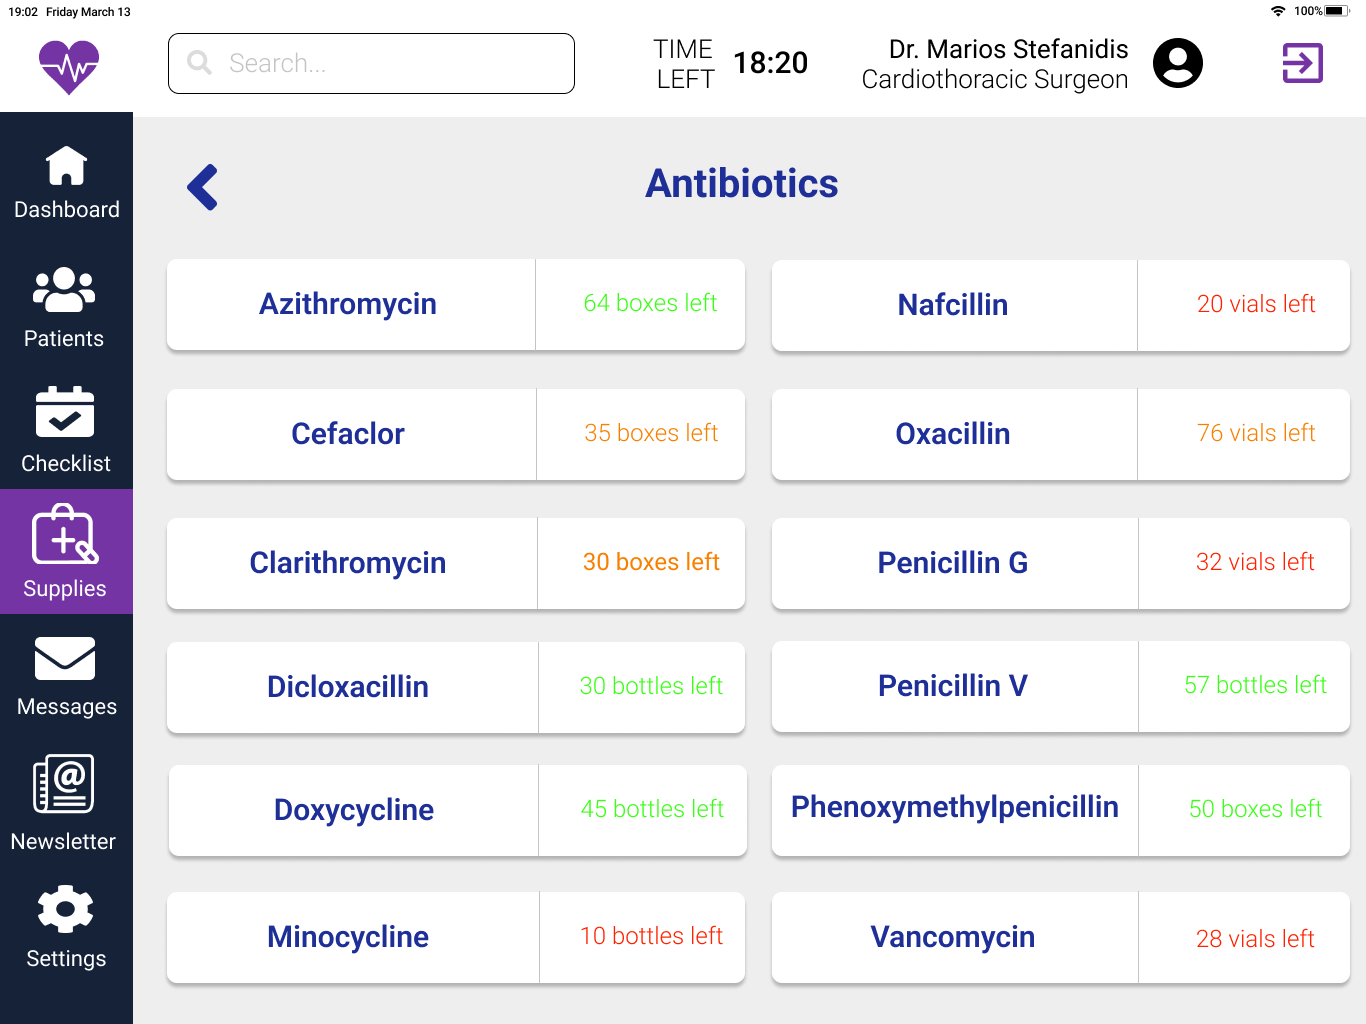
\includegraphics[width=0.5\textwidth]{(Example) Antibiotics Availability.png} 
\caption{\label{fig:antibiotics} Καταχώρηση Νέου Φαρμάκου}
\end{figure}

\subsection{Κεντρική Σελίδα Διαχειριστή Συστήματος}
(*) Σε περιπτώση που συνδεθεί στο \textbf{Medic World} με τους κωδικούς του ένας από τους Διαχειριστές του Συστήματος, θα οδηγηθεί στην εικόνα 20 που θα είναι η αρχική του σελίδα, οι λειτουργίες της οποίας είναι αντίστοιχες με αυτές του γιατρου προσαρμοσμένες στις απαιτήσεις της ειδότητάς του.

\newpage

\begin{figure}[!htb]
\centering
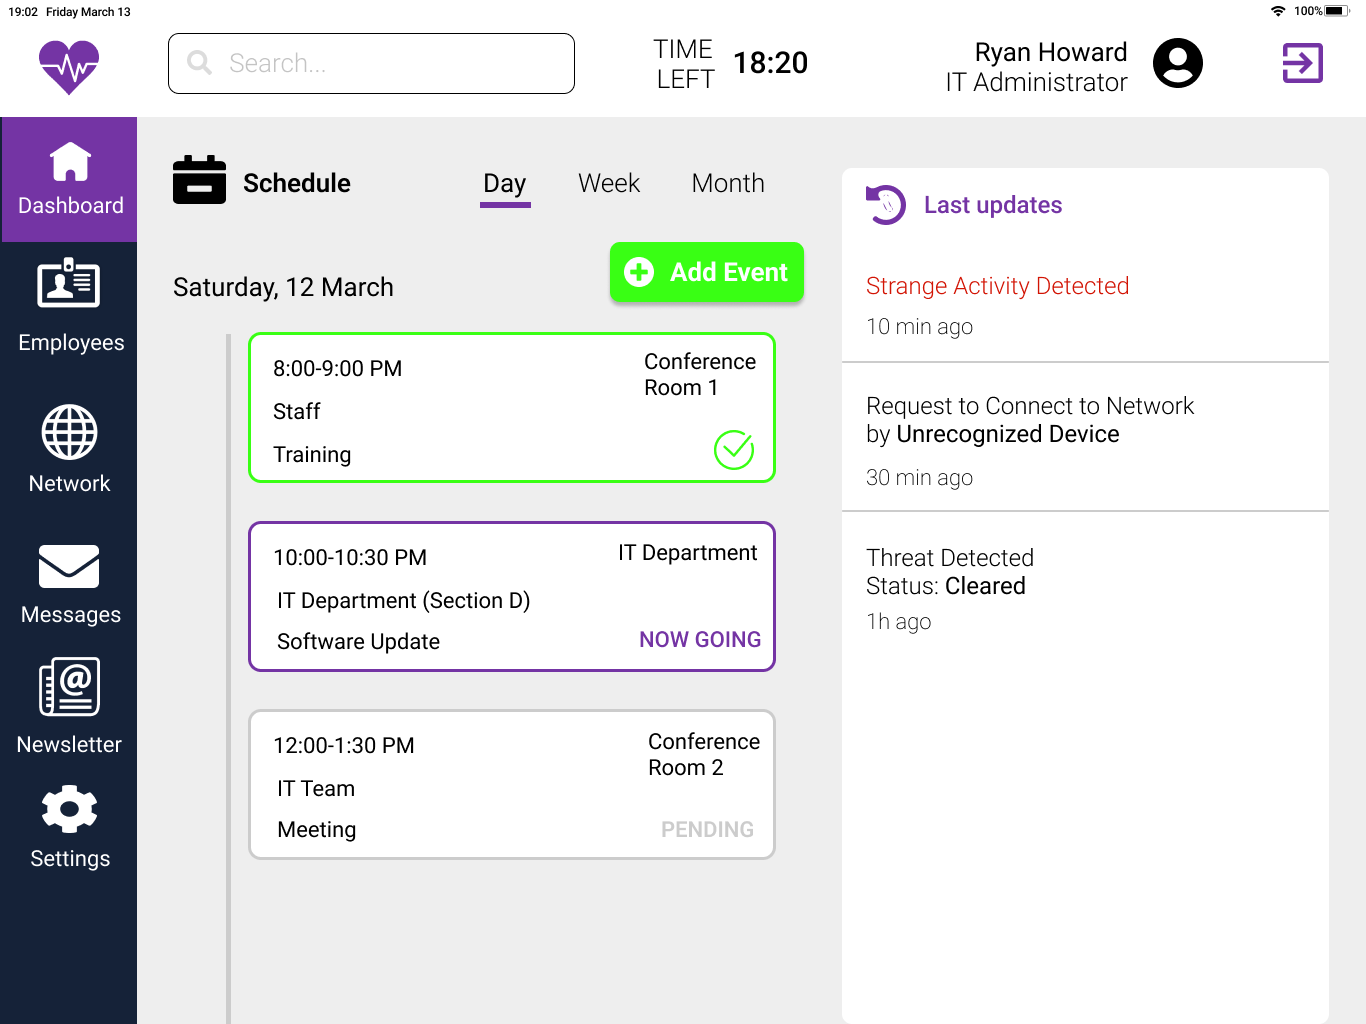
\includegraphics[width=0.5\textwidth]{Dashboar Admin.png} 
\caption{\label{fig:dashboard admin} Κεντρική Σελίδα Διαχειριστή Συστήματος}
\end{figure}

\subsection{Διαχείριση Χρηστών του Συστήματος}

(*) Ο διαχειριστής του συστήματος επιλέγοντας τη λειτουργία "Employee" οδηγείται σε ένα μενού με τις κατηγορίες εργαζομένων του νοσοκομείου του τομέα της ιατροφαρμακευτικής περίθαλψης και επιλέγοντας μία από αυτές (λ.χ. ιατρικό προσωπικό) οδηγείται σε μία καρτέλα, η οποία περιέχει όλους τους εργαζομένους, ενεργούς και μη (με την αντίστοιχη πράσινη και κόκκινη ένδειξη), στο συγκεκριμένο κλάδο (με αλφαβητική σειρά) (εικόνα 21). Μέσω αυτής της οθόνης ο χρήστης έχει τη δυνάτοτητα να επεξεργάζεται τις καρτέλες των εργαζομένων, να προσθέτει, να διαγράφει κ.ο.κ.

\vspace{0.3cm}

\begin{figure}[!htb]
\centering
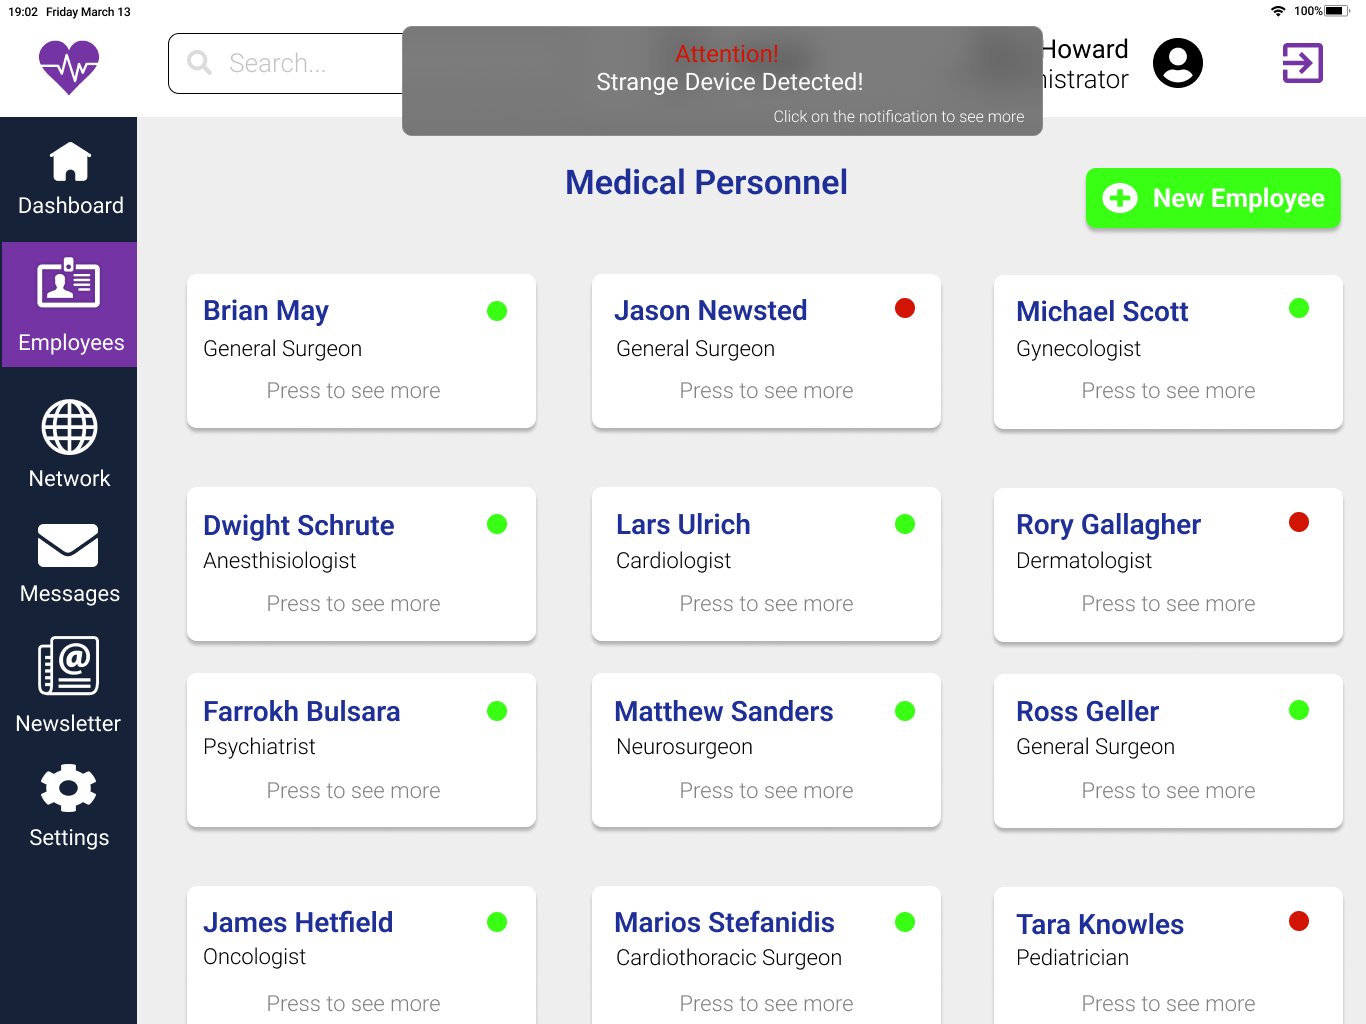
\includegraphics[width=0.5\textwidth]{Employees.png} 
\caption{\label{fig:main page (admin)} Κεντρική Σελίδα Διαχειριστή Συστήματος}
\end{figure}

\subsubsection{Προσθήκη Νέου Υπαλλήλου}

(*) Από την καρτέλα των εργαζομένων (εικόνα 21) μίας κατηγορίας ο διαχειριστής συστήματος επιλέγοντας τη λειτουργία "New Employee" τού δίνεται η δυνατότητα προσθήκης νέου εργαζομένου - χρήστη στο σύστημα (εικόνα 22).


\newpage

\begin{figure}[!htb]
\centering
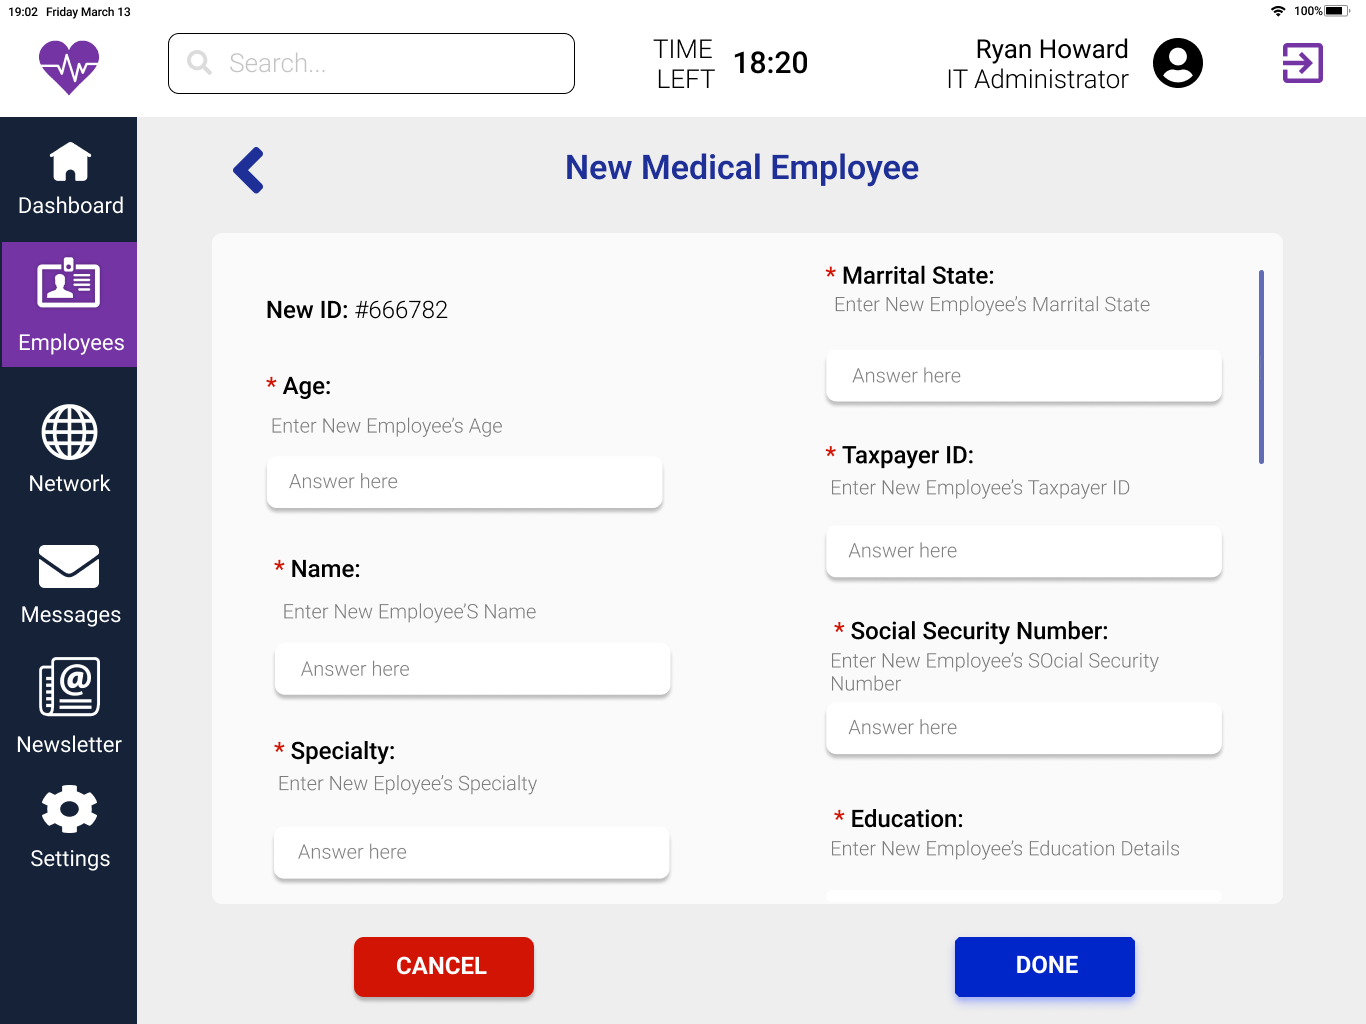
\includegraphics[width=0.5\textwidth]{New Employee.png} 
\caption{\label{fig: new employee} Προσθήκη Νέου Υπαλλήλου}
\end{figure}

\subsection{Καρτέλα Διαχείριση Δικτύου}

(*) Επιλέγοντας τη λειτουργία "Network" ο χρήστης οδηγείται σε ένα μενού, το οποίο του παρέχει τη δυνατότητα ελέγχου και διαχείρισης δικτύου (εικόνα 23).

Οι επιλογές που δίνονται στην καρτέλα διαχείρισης δικτύου αναγράφονται παρακάτω:
\begin{itemize}
    \item Check Devices: στο χρήστη παρέχεται μία λίστα με τα ονόματα, τον τρόπο σύνδεσης, τις διευθύνσεις IPv4 και MAC των συσκευών, καθώς και μία ένδειξη επικινδυνότητας (κόκκινα και πράσινα κυκλάκια). Περισσότερα για τη συγκεκριμένη ένδειξη παρουσιάζονται στην ενότητα 3.11.1
    \item Check Users: μέσω της συγκεκριμένης λειτουργίας ο διαχειριστής του συστήματος μπορεί να ελέγξει τις κινήσεις των χρηστών στο δίκτυο και στην εφαρμογή
    \item Check Network: ο χρήστης μπορεί να επιβλέπει τις λεπτομέρειες του δικτύου, όπως bandwidth, traffic, strength κ.ο.κ.
    \item Manage Network: ο administrator διαχειρίζεται το δίκτυο. Από εδώ θα μπορεί να διαγράψει συσκευές και να επεξεργαστεί τις πληροφορίες που αφορούν το δίκτυο
\end{itemize}

\begin{figure}[!htb]
\centering
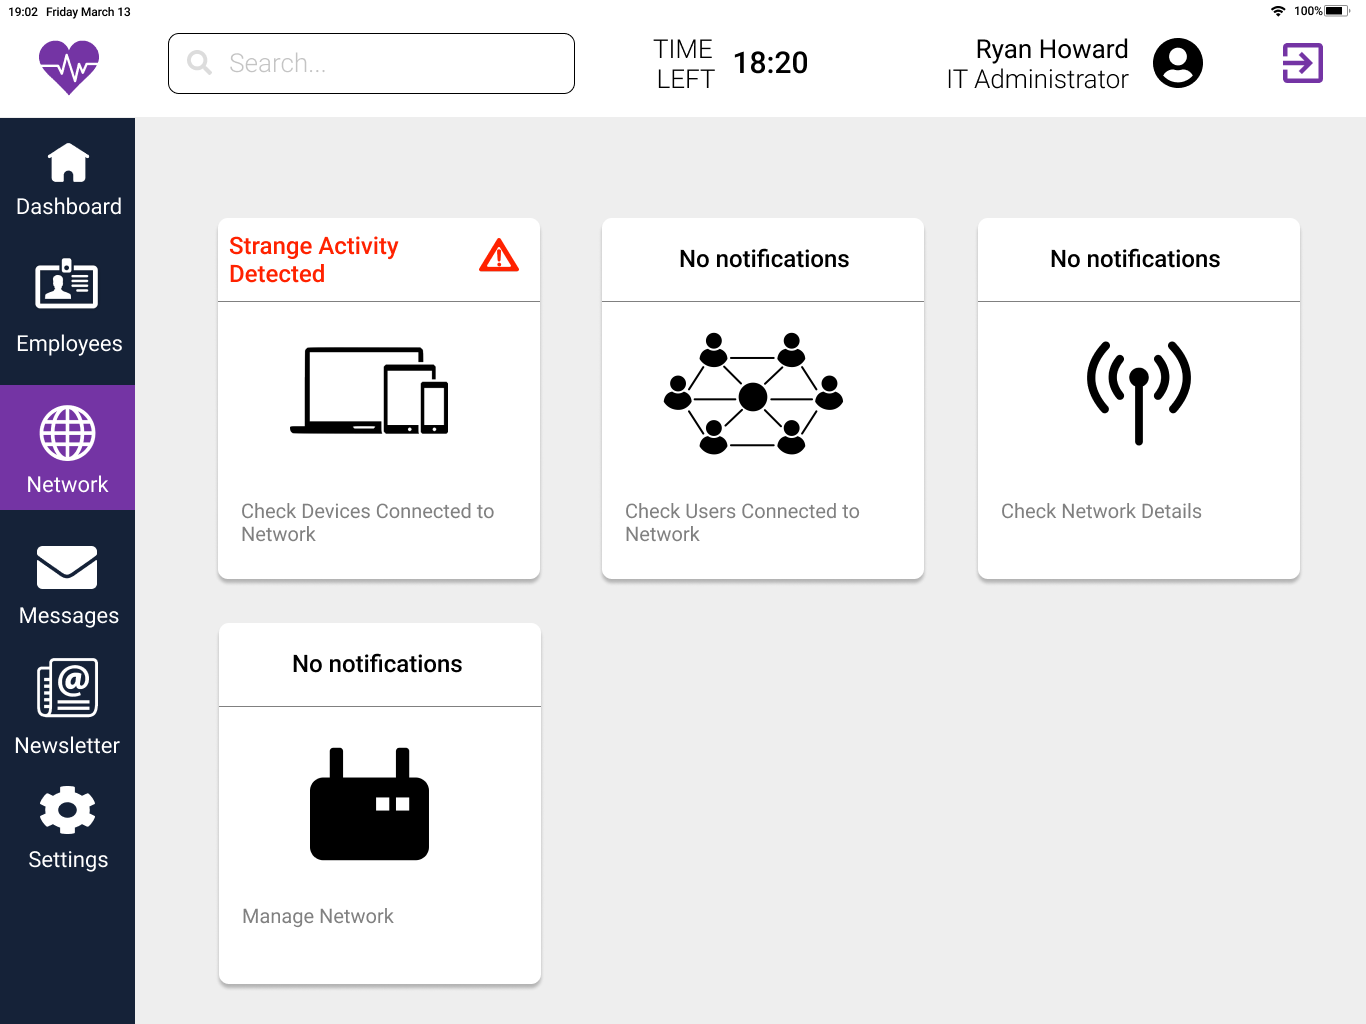
\includegraphics[width=0.5\textwidth]{Network Monitoring.png} 
\caption{\label{fig:netowrk monitoring} Καρτέλα Διαχείρισης Δικτύου }
\end{figure}

\subsubsection{Διαχείριση Δικτύου}

(*) Από το μενού διαχείρισης επιλέγοντας να ελέγξει τις συσκευές που είναι συνδεδεμένες στο δίκτυο, το \textbf{Medic World} παρέχει μία λίστα με τα ονόματα, τον τρόπο σύνδεσης, τις διευθύνσεις IPv4 και MAC των συσκευών, καθώς και μία ένδειξη επικινδυνότητας (κόκκινα και πράσινα κυκλάκια) (εικόνα 24).Από την παραπάνω λίστα ο χρήστης μπορεί  να επιλέξει κάποια από τις εμφανιζόμενες συσκευές και να ελέγξει τις κινήσεις της ή και να την απομακρύνει από το δίκτυο.


\begin{figure}[!htb]
\centering
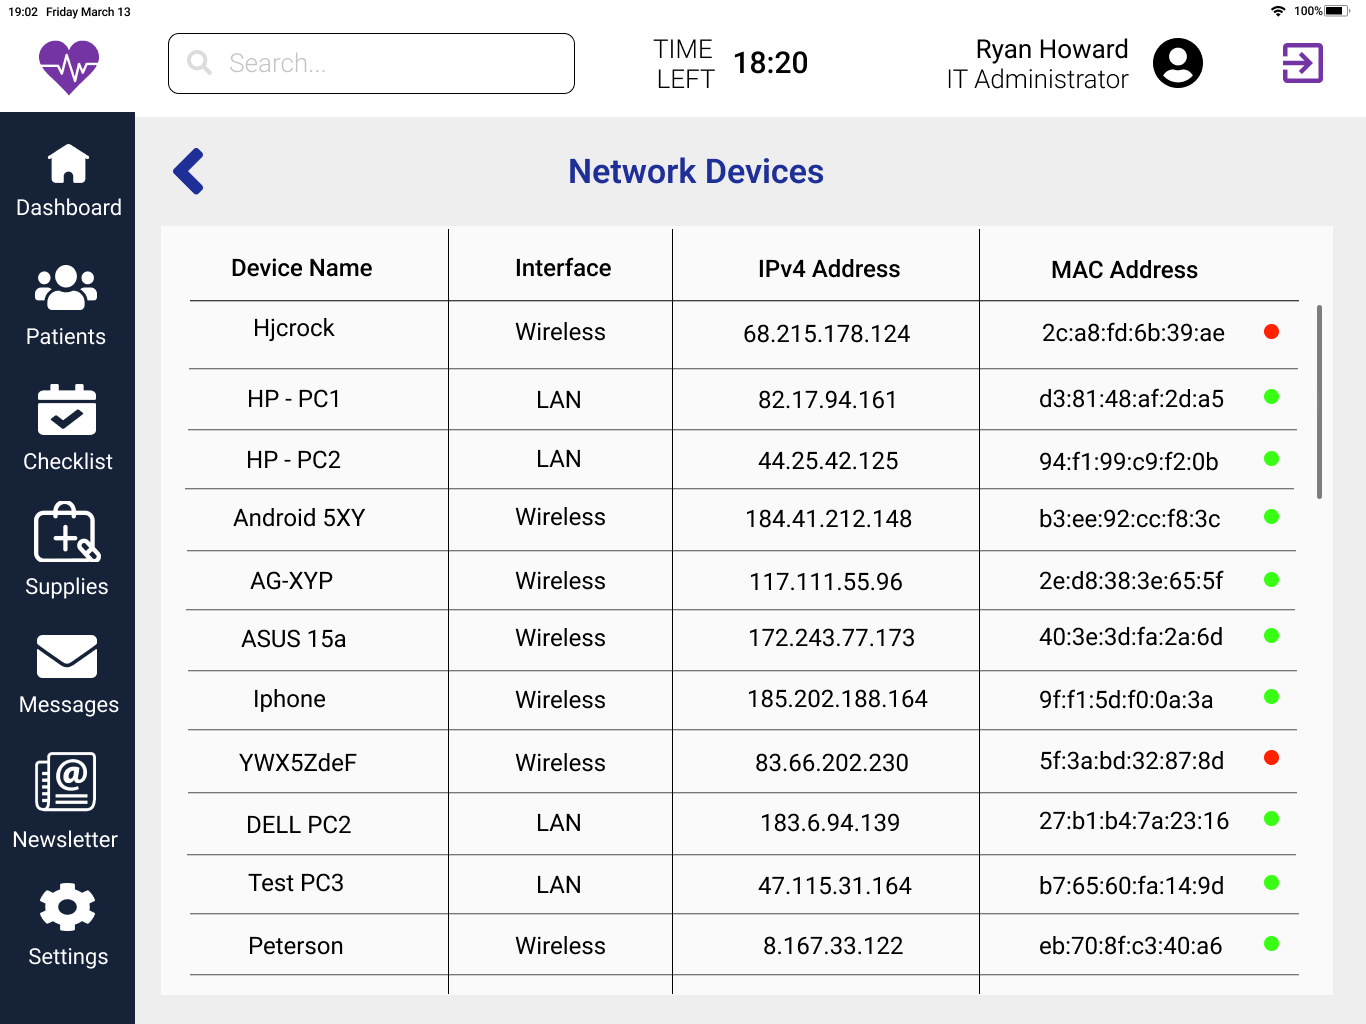
\includegraphics[width=0.5\textwidth]{Devices.png} 
\caption{\label{fig: devices} Διαχείριση Συσκευών Δικτύου}
\end{figure}

\subsection{Μηνύματα}

(*) Μέσω της καρτέλας "Messages" (εικόνα 25) όλοι οι χρήστες έχουν τη δυνατότητα επικοινωνίας με οποιονδήποτε είναι συνδεδεμένος στο \textbf{Medic World} (ανήκει στο προσωπικό). 

\vspace{0.3cm}

\textbf{Σημείωση:} Για το design της καρτέλας messages έχουμε βασιστεί στο design της εφαρμογής \\ messenger.

\vspace{0.3cm}

\begin{figure}[!htb]
\centering
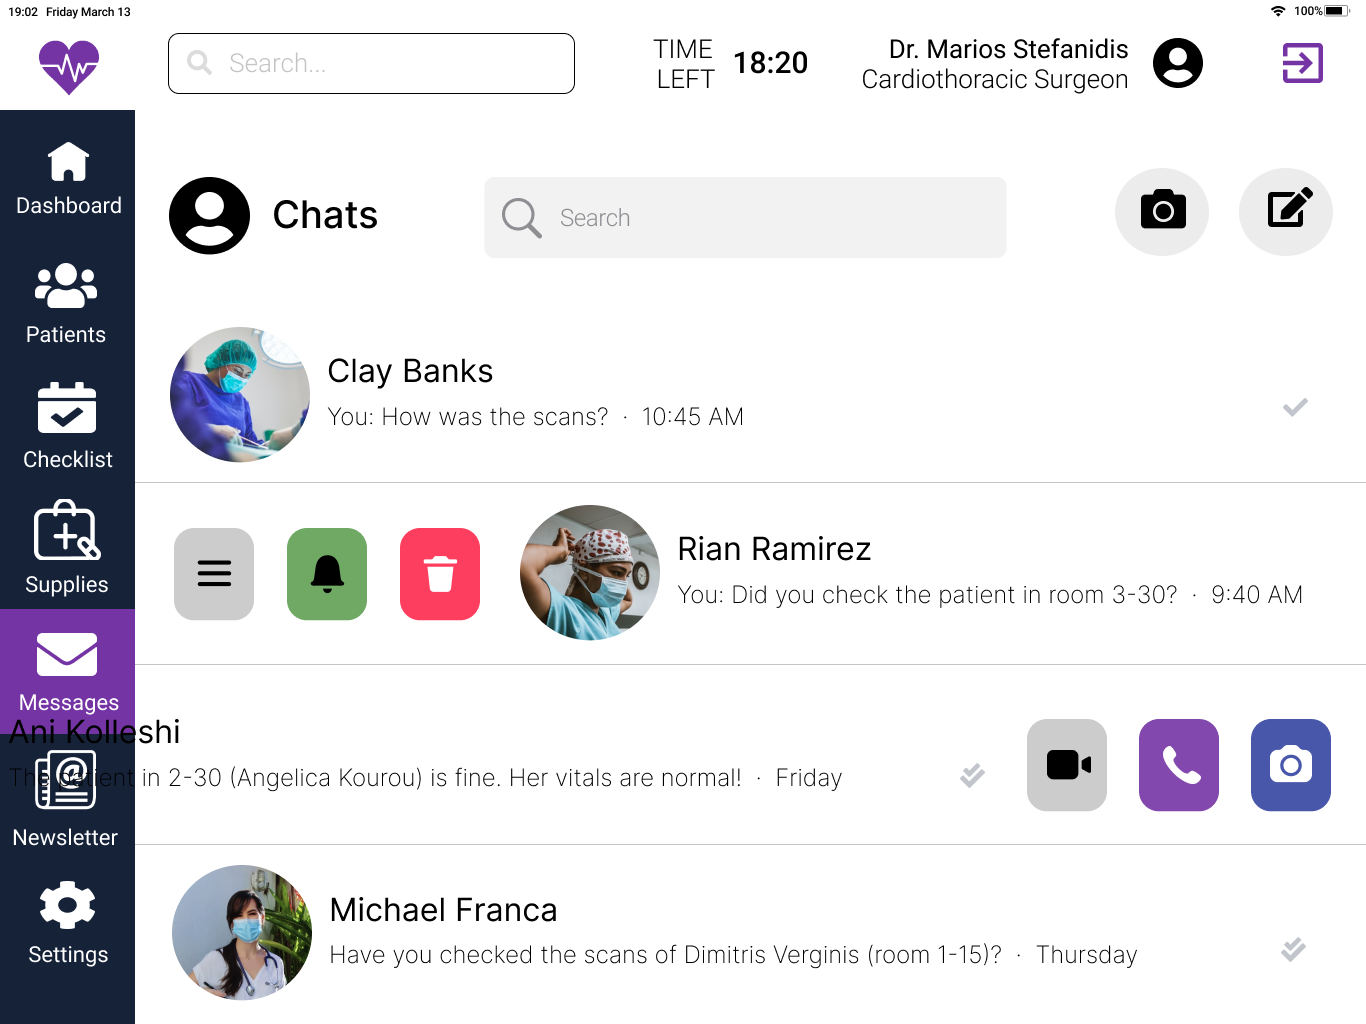
\includegraphics[width=0.5\textwidth]{Messages (1).png} 
\caption{\label{fig: messenger} Καρτέλα Συνομιλιών}
\end{figure}

\newpage

\par Με τις λειτουργίες swipe right/left (εικόνα 26) θα εμφανίζονται στο χρήστη δυνατότητες  που αφορούν τη διαγραφή συνομιλιών, δημιουργία βιντεοκλήσης κ.ο.κ. 

\vspace{0.3cm}

\begin{figure}[!htb]
\centering
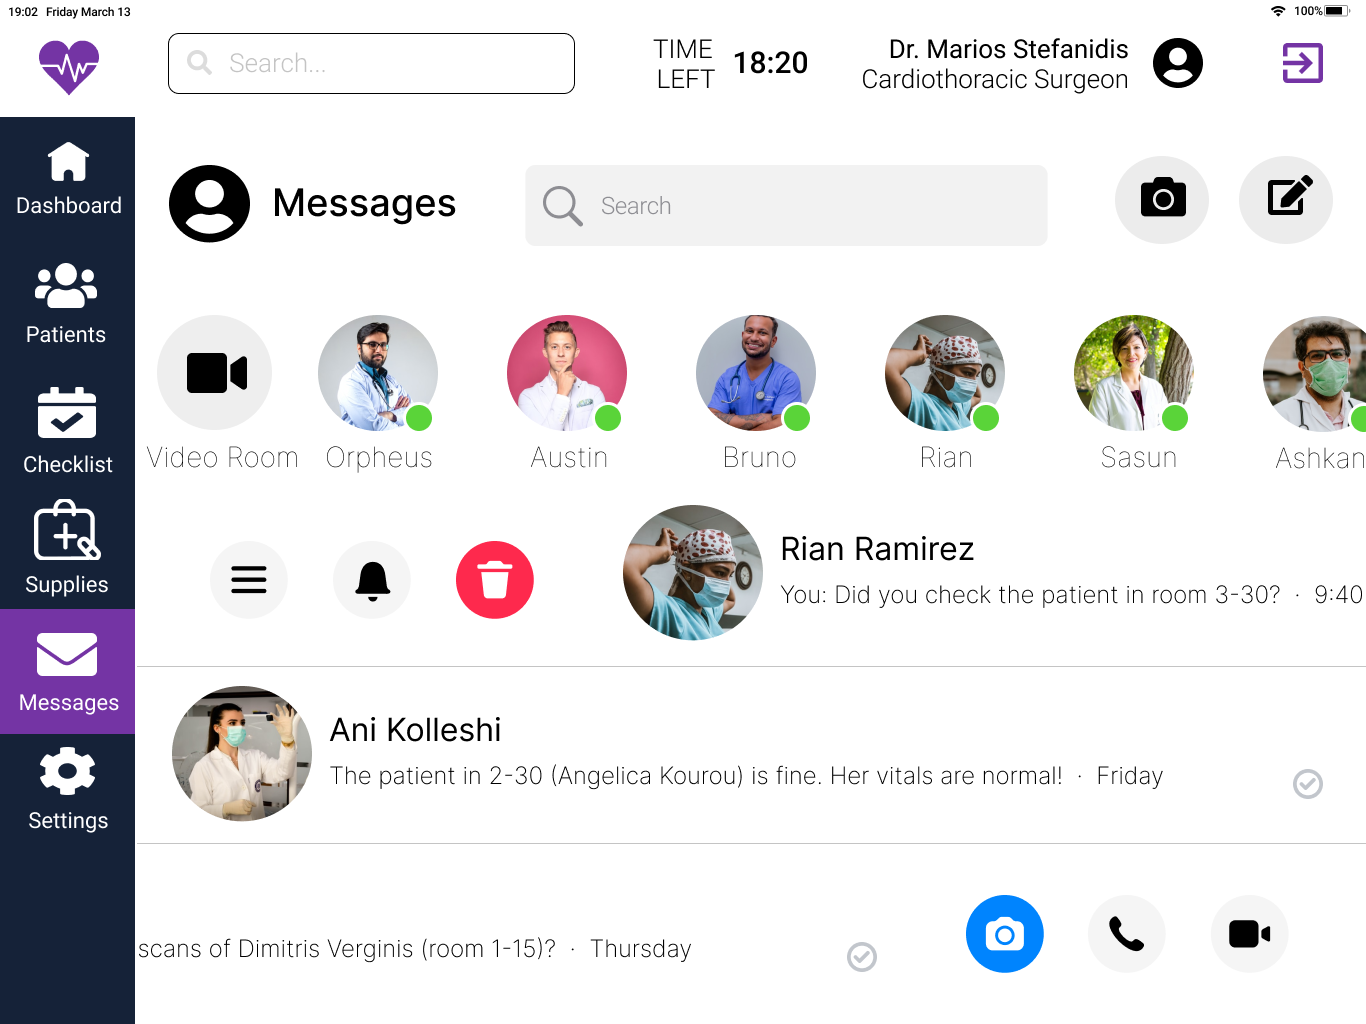
\includegraphics[width=0.5\textwidth]{Messages (actions).png} 
\caption{\label{fig: swipe left/right} Λειτουρργίες Συνομιλιών}
\end{figure}

\subsubsection{Συνομιλίες}

Από την καρτέλα συνομιλιών (εικόνα 25) επιλέγοντας είτε κάποια εικόνα προφίλ είτε κάποια από τις συνομιλίες, ο χρήστης οδηγείται στο συγκεκριμένο προσωπικό chat (εικόνα 26). Κάποιες από τις λειτουργίες που παρέχονται είναι η ηχογράφηση μηνύματος, αποστολή εργαστηριακών εξετάσεων ή κάποιας φωτογραφίας κ.ο.κ.

\vspace{0.3cm}

\begin{figure}[!htb]
\centering
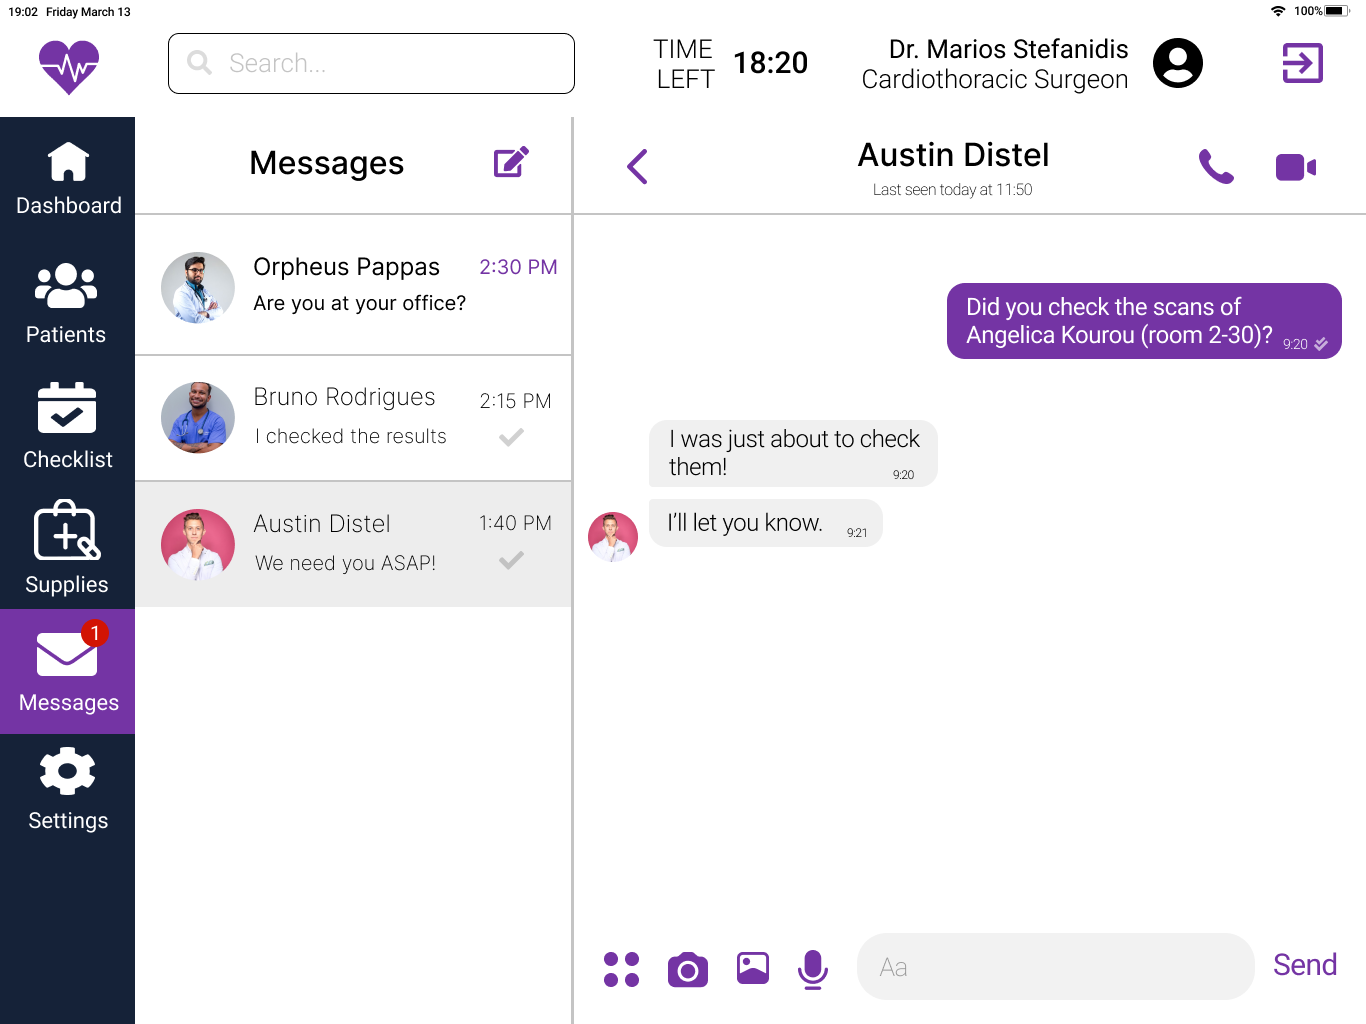
\includegraphics[width=0.5\textwidth]{Messages (discussion).png} 
\caption{\label{fig: discussion} Προσωπική Συνομιλία}
\end{figure}

\subsection{Newsroom}

(*) Η λειτουργία Newsroom προσφέρει στους χρήστες του \textbf{Medic World} υπηρεσίες ανάλογες με αυτές εφαρμογών κοινωνικής δικτύωσης, όπως η παροχή άρθρων σχετικών με τις εξελίξεις του ιατρικού τομέα, η δημοσίευση ερωτήσεων και ανακοινώσεων μεταξύ των χρηστών και η δημιουργία εκδηλώσεων σχετικών με την επαγγελματική τους απασχόληση.

\newpage

\subsubsection{News Article}

Μέσω της συγκεκριμένης καρτέλας (εικόνα 28) οι χρήστες μπορούν να πλοηγούνται και να ανακαλύπτουν άρθρα σχετικά με τα επαγγελματικά τους ενδιαφέροντα, τα οποία θα έχουν τη δυνατότητα να κοινοποιούν είτε μέσω της εφαρμογής είτε μέσω ηλεκτρονικού ταχυδρομείου, να αποθηκεύουν ώστε να τα αναζητούν αργότερα και να αποκρύπτουν όταν δεν τους ενδιαφέρουν.

\vspace{0.3cm}

\textbf{Σημείωση:} Τα άρθρα θα επιλέγονται μέσω ειδικού αλγόριθμου με βάση την επαγγελματική ιδιότητα των χρήστων αλλά και τις προηγούμενες αναζητήσεις τους.

\vspace{0.3cm}

\begin{figure}[!htb]
\centering
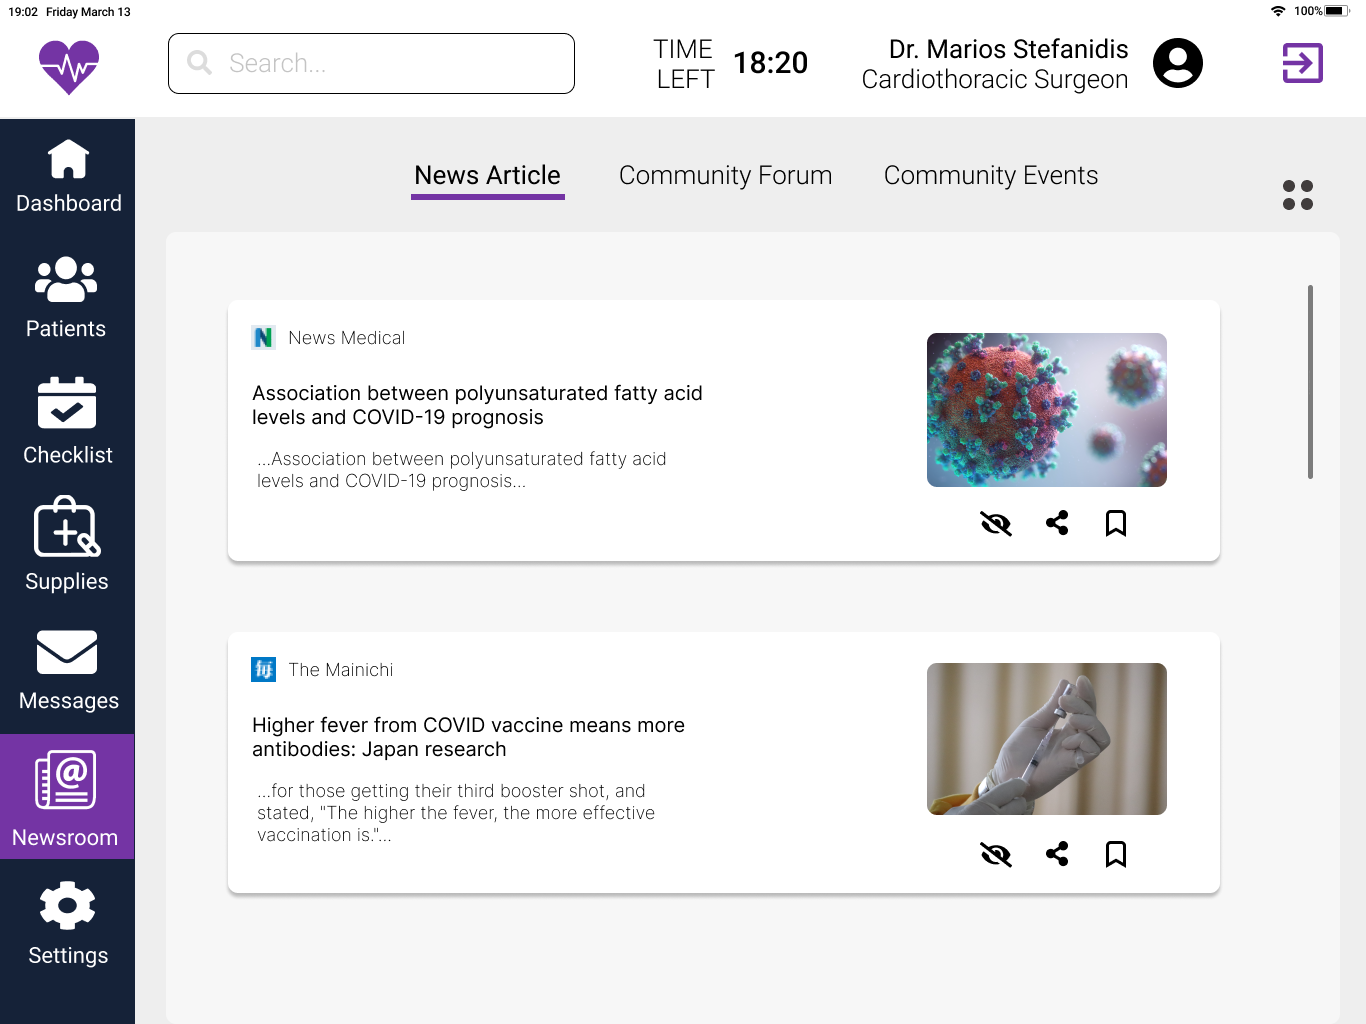
\includegraphics[width=0.5\textwidth]{Articles.png} 
\caption{\label{fig: news article} News Article}
\end{figure}

\subsubsection{Community Forum}

Στο Community Forum (εικόνα 29) στους χρήστες του \textbf{Medic World} παρέχεται η δυνατότητα για δημοσίευση post που θα αφορούν νοσοκομειακά/ιατρικά θέματα. Τα post πριν την τελική τους δημοσιοποίηση θα απαιτούν έγκριση από το διαχειριστή του συστήματος, ώστε το περιεχόμενο τους να μην παρεκκλίνει από το πλαίσιο που έχει καθοριστεί.

\vspace{0.3cm}

\begin{figure}[!htb]
\centering
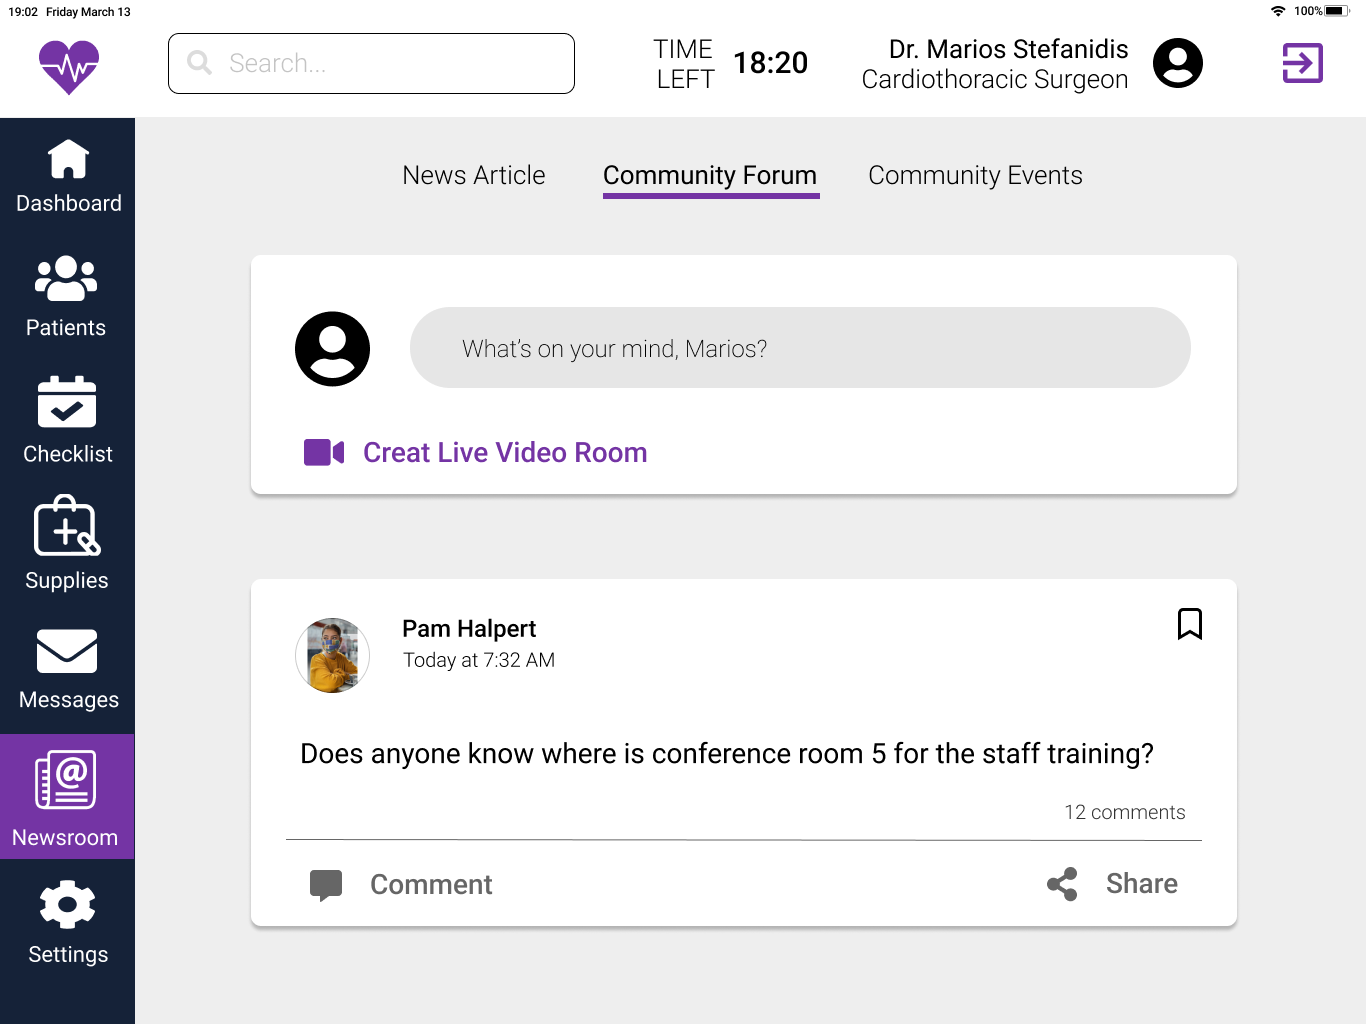
\includegraphics[width=0.5\textwidth]{Community Forum.png} 
\caption{\label{fig: community forum} Community Forum}
\end{figure}

\newpage

\subsubsection{Community Events}

Στο Community Events (εικόνα 30) εμφανίζονται στους χρήστες οι διάφορες εκδηλώσεις που έχουν αναρτηθεί στο \textbf{Medic World}, όπου ο χρήστης θα μπορεί να δηλώσει ενδιαφέρον συμμετοχής.

\begin{figure}[!htb]
\centering
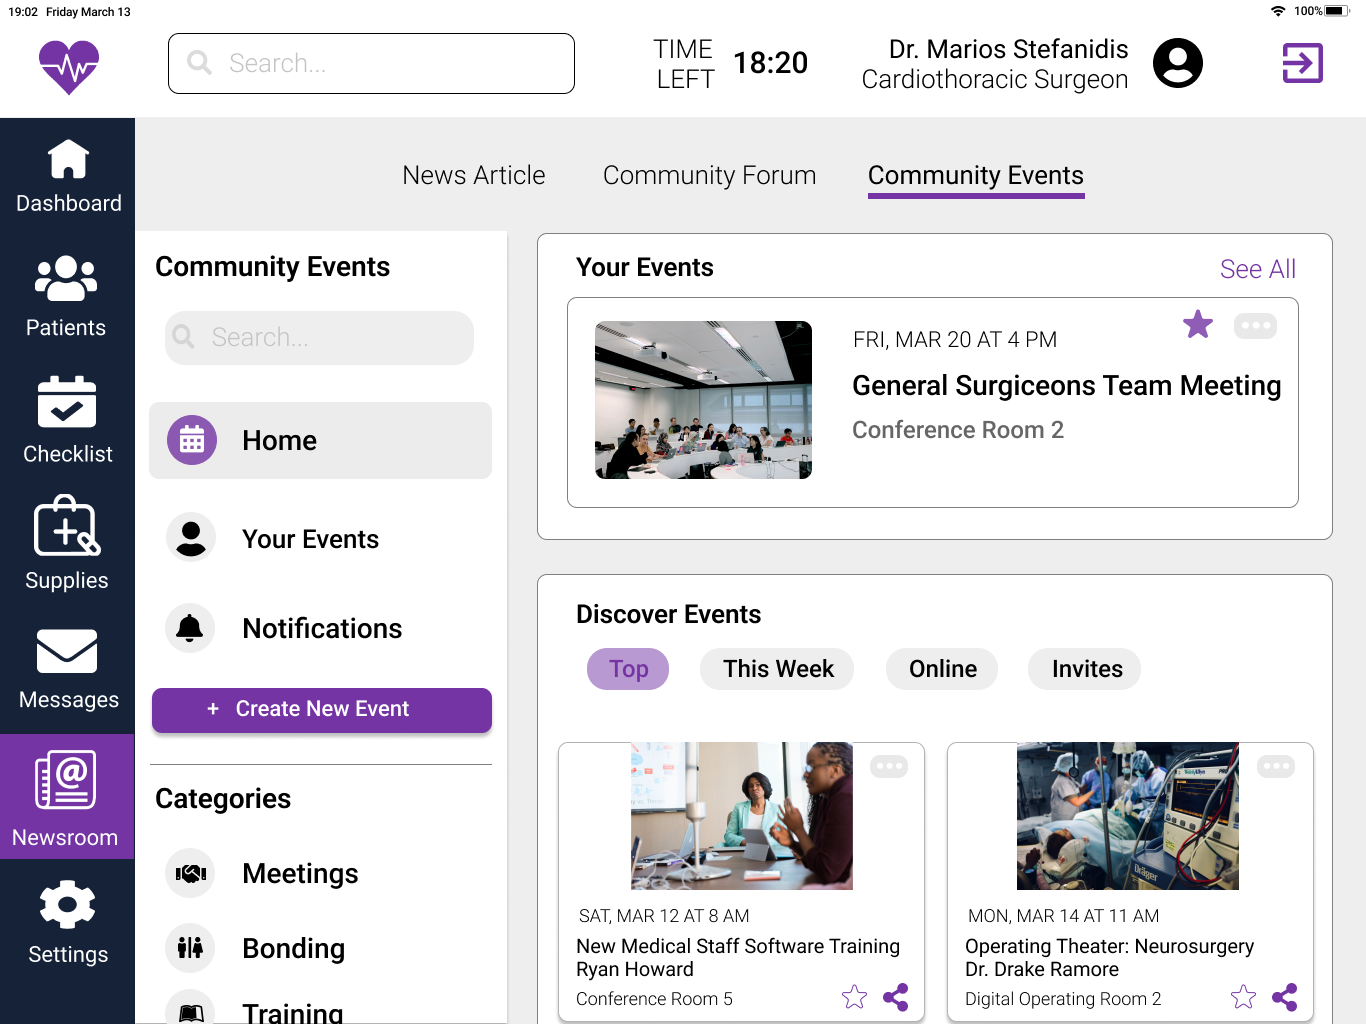
\includegraphics[width=0.5\textwidth]{Community Events.png} 
\caption{\label{fig: community events} Community Events}
\end{figure}

\subsubsection{Δημιουργία Εκδήλωσης}

Το \textbf{Medic World} παρέχει την λειτουργία "Create New Event", μέσω της οποίας οι χρήστες μπορούν να δημιουργήσουν εκδηλώσεις (ιατρικά σεμινάρια, συναντήσειςεκπαίδευση προσωπικού) συμπληρώνοντας τα απαραίτητα στοιχεία.
\par Στην εικόνα 31 παρέχεται στον χρήστη η δυνατότητα είτε δια ζώσης είτε εξ αποστάσεως διεξαγωγής της εκδήλωσης.

\vspace{0.3cm}

\begin{figure}[!htb]
\centering
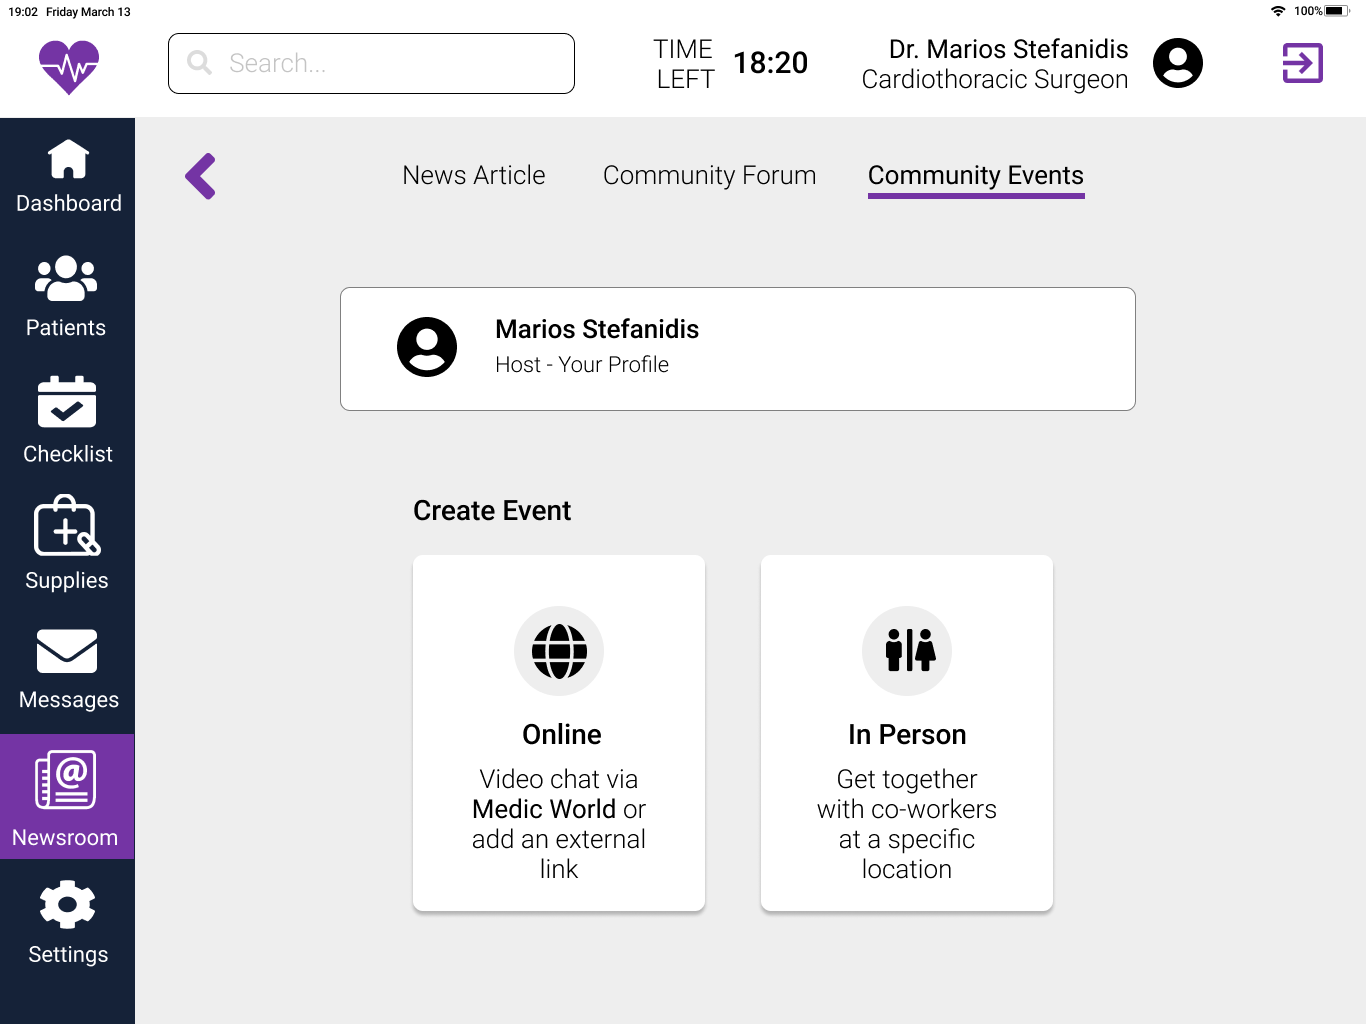
\includegraphics[width=0.5\textwidth]{Create event 1.png} 
\caption{\label{fig: event1} Τρόπος Διεξαγωγής της Εκδήλωσης}
\end{figure}

\newpage

\par Στις εικόνες 32, 33 και 34 συμπληρώνονται οι απαραίτητες πληροφορίες για την δημουργία της εκδήλωσεις όπως είναι η τοποθεσία, η ημερομηνία κ.ο.κ.

\begin{figure}[!htb]
\centering
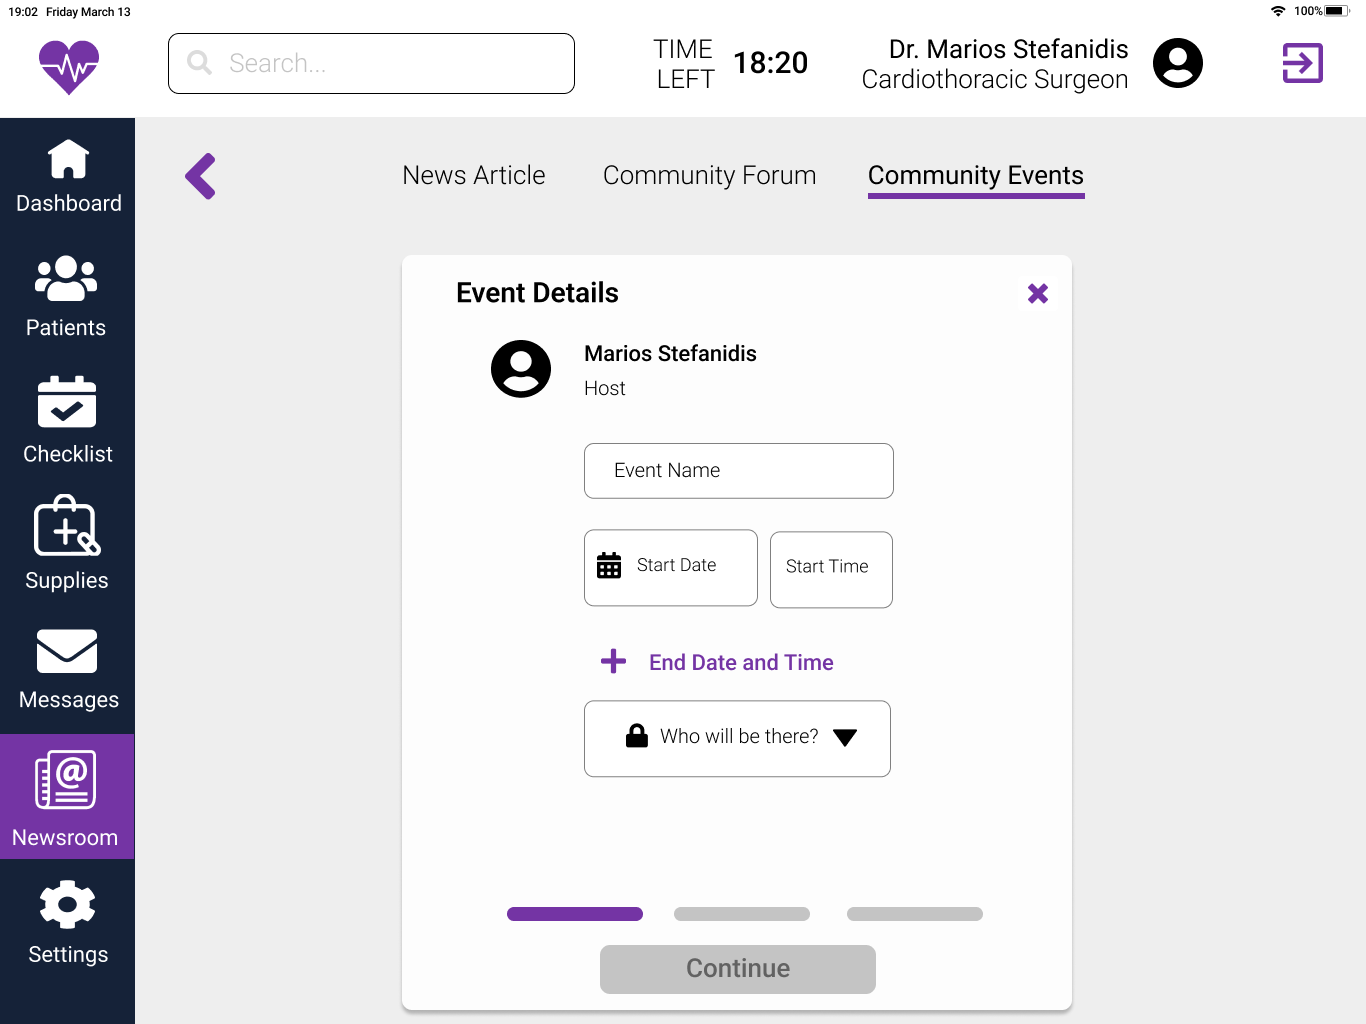
\includegraphics[width=0.5\textwidth]{Create event 2.png} 
\caption{\label{fig: event2} Δημιουργία Εκδήλωσης - Βήμα 1}
\end{figure}

\vspace{0.3cm}

\begin{figure}[!htb]
\centering
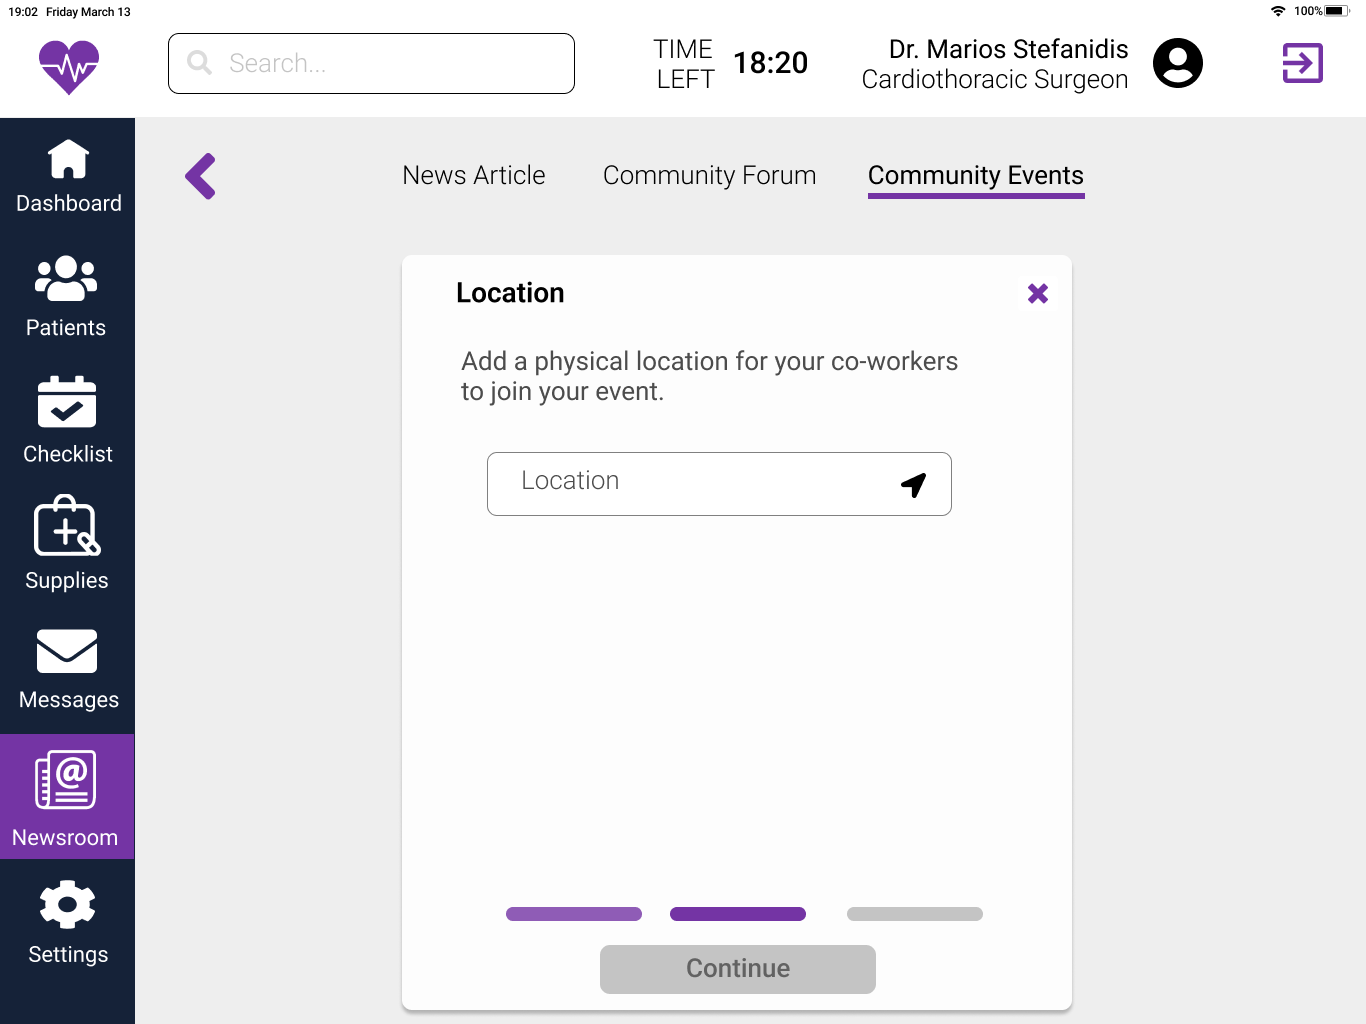
\includegraphics[width=0.5\textwidth]{Create event 3.png} 
\caption{\label{fig: event3} Δημιουργία Εκδήλωσης - Βήμα 2}
\end{figure}

\vspace{0.3cm}

\begin{figure}[!htb]
\centering
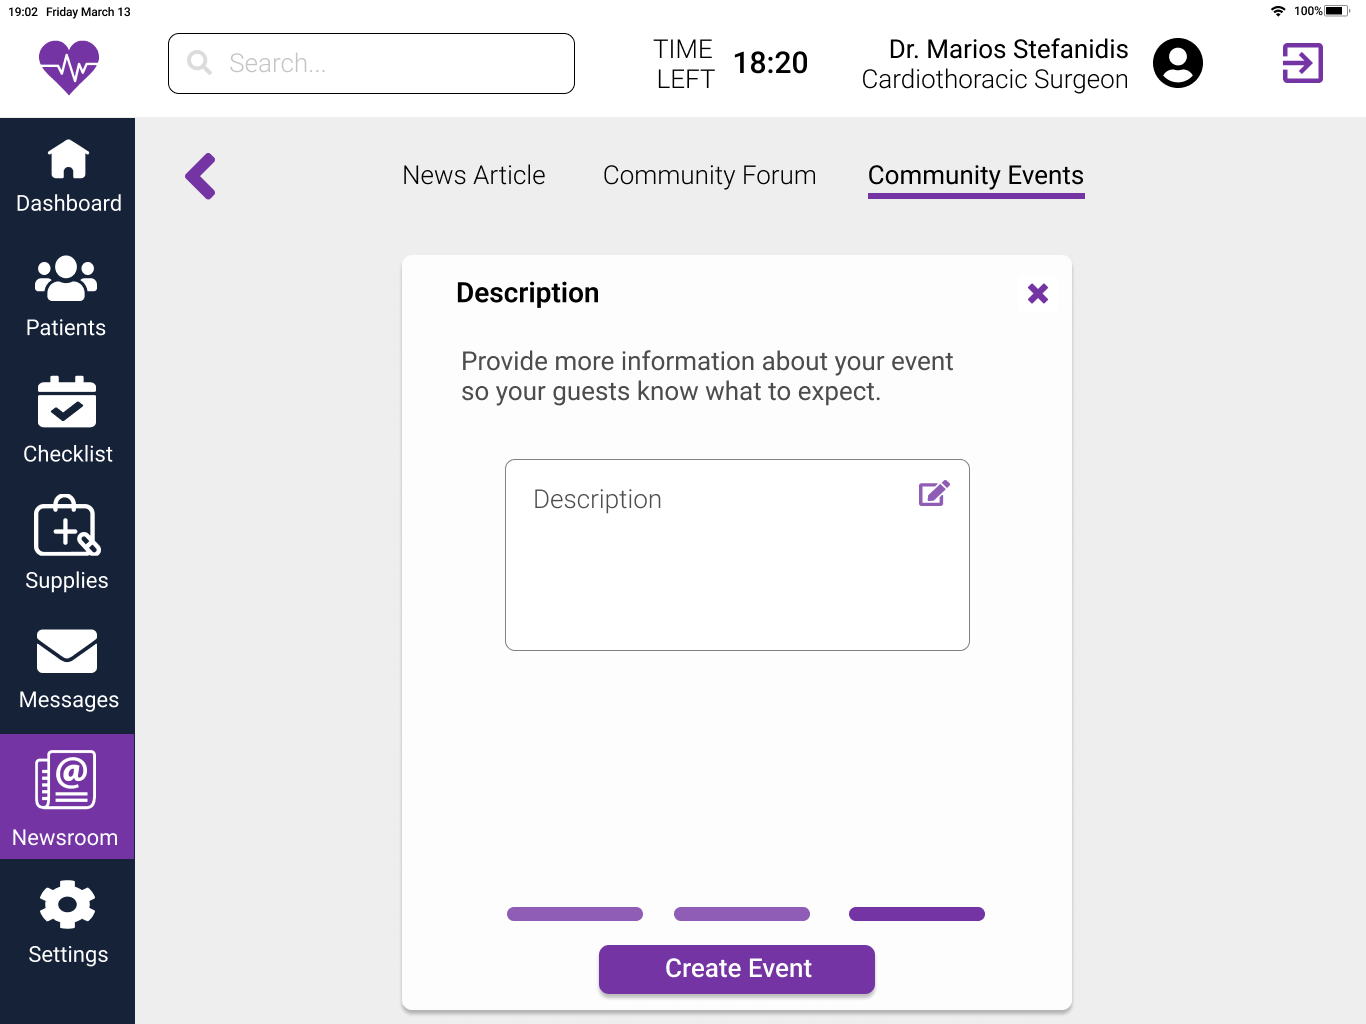
\includegraphics[width=0.5\textwidth]{Create event 5.png} 
\caption{\label{fig: event4} Δημιουργία Εκδήλωσης - Βήμα 3}
\end{figure}


\end{document}
